%\documentclass[preprint,3p,times,twocolumn]{elsarticleUS}
\documentclass[review,3p,times]{elsarticleUS}
\usepackage{amssymb}
\usepackage{amsmath}
\usepackage{graphicx}
\usepackage{bm}
\usepackage{yhmath}
\usepackage{subfigure}
\usepackage{multirow}
\usepackage{cleveref}
\usepackage{color}
\usepackage{xcolor}
\usepackage{subdepth}
\usepackage[nomarkers,lists]{endfloat}

\def\pp#1#2{\frac{\partial #1}{\partial #2}}

\biboptions{comma,sort&compress}

\journal{Combustion and Flame}

\makeatletter
\def\@author#1{\g@addto@macro\elsauthors{\normalsize%
    \def\baselinestretch{1}%
    \upshape\authorsep#1\unskip\textsuperscript{%
      \ifx\@fnmark\@empty\else\unskip\sep\@fnmark\let\sep=,\fi
      \ifx\@corref\@empty\else\unskip\sep\@corref\let\sep=,\fi
      }%
    \def\authorsep{\unskip,\space}%
    \global\let\@fnmark\@empty
    \global\let\@corref\@empty  %% Added
    \global\let\sep\@empty}%
    \@eadauthor={#1}
}
\makeatother

\begin{document}

\begin{frontmatter}

\title{Autoignition-affected stabilization of laminar nonpremixed DME/air coflow flames}

\author{Sili~Deng\corref{cor}}
\author{Peng~Zhao}
\author{Michael E.~Mueller}
\author{Chung K.~Law}
\cortext[cor]{Corresponding Author: silideng@princeton.edu}

\address{Department of Mechanical and Aerospace Engineering, Princeton University, Princeton, NJ 08544, USA}

\begin{abstract}

The structure and stabilization mechanism of laminar nonpremixed autoignitive DME/air coflow flames were investigated under typical gas turbine conditions.  The simulations were performed at $30$ atmospheres with uniform inlet velocity of $3.2$ m/s for both streams, and the coflow air boundary temperatures were $700$, $800$, $900$, and $1100$ K.  The heat release and species profiles of each case were examined. Further investigation with Chemical Explosive Mode Analysis (CEMA) and Lagrangian Flamelet Model (LFM) were performed to identify the controlling chemistry and elucidate the combustion mode and stabilization mechanism.  At $700$ to $900$ K, autoignition was demonstrated to be the dominant stabilization mechanism, and the NTC chemistry determines the stabilization point in mixture fraction space.  Moreover, the coupling between the autoignition process and premixed flame propagation results in the multibrachial structure.  On the other hand, at $1100$ K, the kinematic balance between the premixed flame propagation velocity and the incoming flow velocity becomes the dominating stabilization mechanism, and the classical triple flame structure was observed.  Extended stabilization regimes, in terms of increasing boundary temperature, was therefore identified, including the frozen flow, purely kinetically stabilized, autoignition-propagation-coupling stabilized, purely kinematically stabilized, and burner stabilized regimes.           

\end{abstract}

\begin{keyword} 
Dimethyl ether (DME) \sep Autoignition \sep Stabilization \sep Nonpremixed coflow flame \sep Negative Temperature Coefficient (NTC)
\end{keyword}

\end{frontmatter}


%\clearpage % For word count
\section{Introduction}

Nonpremixed jet flames have been extensively studied to understand the combustion processes in diesel engines.  The stabilization and structure of the jet flames determine the lifted height of the flame, therefore is crucial to the engine design.  Due to the mixing process of the fuel and oxidizer streams, the combustion mode is partially premixed, resulting in a two-dimensional tribracial flame~\cite{buckmaster02}, namely, a lean and a rich premixed flame wing with a trailing diffusion flame branch.  The point where the three branches intersect is called the triple point and is generally considered as the stabilization point for nonautoignitive cases. The dynamic balance bewteen the local flame propagation speed and incoming flow speed is characterized as the stabilization mechanism.  A recent review by Chung~\cite{chung07} discussed the stabilization, propagation and instability of tribrachial flames, including the the effects of concentration gradient~\cite{17-19}, velocity gradient~\cite{37}, and burnt gas expension~\cite{14,25-27}.  Details about the referred experimental observations and computational simulations can be found in the literatures therein. These studies, however, limited to the nonautoignitive conditions, while the real diesel engine is operated at elevated pressures and temperatures, where autoignitions are activated and might interact with the tribracial flame. 

Chung and co-workers~\cite{choi09,choi10,choi12} conducted a series of experiments to investigate the autoignition characteristics of laminar C$_1$ to C$_4$ fuel jets in a heated coflow air jet and found that above certain coflow temperatures, lifted flames could be estabilished through autoignitions.  In these studies, both the tribrachial structure for most autoignited cases and a repetitive behavior of extinction and reignition at the critical condition near blowout were observed.  However, the role that autoignition plays in the stabilization mechanism as well as its influences on the tribrachial flame is still less understood.  

Furthermore, diesel fuels have two-stage ignition processes, where the first stage ignition is governed by the low temperature chemistry, and the second stage ignition is dominated by the high temperature chemistry.  In both low and high temperature regimes, the ignition delay time decreases as the intial temperature increases.  However, in the intermediate temperature regime, the transition of the ignition results in increased overall iginition delay time as the initial temperature increases.  Therefore, this nonmonotonic response of the ignition delay time to increasing initial temperature is referred as the negative temperature coefficient (NTC), which has been extensively studied in homogeneous system, as it is a major feature of large hydrocarbon autoignition characteristics.  Recently, a series of both computational and experimental studies adopting the nonpremixed counterflow configuration by Law and co-workers~\cite{law12,zhao13,deng14} have demonstrated that with the existence of nonuniformities in the flow, species, and temperature fields, the ignition characteristics of the nonpremixed flames can be fundamentally affected by the low temperature chemistry, especially at elevated pressures and/or reduced strain rates.   

Therefore, the NTC-affected stabilization of nonpremixed lifted flames can be potentially important, yet few literatures provide detailed analysis.  Krisman \emph{et al.}~\cite{krisman14} recently conducted a numercial study of the dimethyl ether (DME)/air mixing layer at $40$ atmospheres and a temperature range of $700$ to $1500$ K and observed polybrachial structures in the heat release profiles.  The mixture fractions corresponding to the stabilization points defined based on the hydroxyl radical (OH) mass fraction and the the first stage autoignition kernels based on the methoxymethylperoxy radical (CH$_3$OCH$_2$O$_2$) were compared with the most reactive mixture fractions computed from homogeneous autoignitions under the same intial conditions.  The transport budget analysis based on selected species was performed to differentiate deflagrations from autoignitions.

The previous study on the polybrachial structure is intriguing, showing the modified flame shape from autoignition in the mixing layer.  However, further investigation should be made to study the detailed chemical structure and stabilization mechanism of the polybrachial flame.  For example, tools for computational diagnostics, especially for dominating reaction identifications at local positions, are needed to understand the controlling chemistry.  On the other hand, considering the two-dimensional structure as well as the thermal and concentration stratification in the mixing layer, a direct comparison to the homogeneous autoignition is unable to distinguish the mixture fraction stratification effects across the mixture fraction iso-contour and the flame back diffusion effects along the mixture fraction iso-contour on the autoignition front.  These considerations would significantly improve the understanding of the role of autoignition in the upstream of the flame structure and quantitatively identify the controlling kinetics and stabilization mechanism.     

In the present study, nonpremixed DME/air coflows were simulated at $30$ atmospheres with the oxidizer stream heated to activate autoignition.  As a clean biofuel and one of the smallest hydrocarbon exhibiting NTC, detailed reaction models for low and high temperature DME oxidation~\cite{curran98,fischer00,curran00,zhao08} have been extensively developed and validated for burner stabilized flames~\cite{kaiser00}, nonpremixed counterflow flame ignition~\cite{zheng05}, laminar flame speeds~\cite{qin05}, allowing for moderate confidence in our computation.  In particular, the present computation was conducted using a skeletal mechanism of $39$ species~\cite{bansal11}, including both low and high temperature oxidation pathways, which is reduced from the well validated detailed mechanism of Zhao \emph{et al.}~\cite{zhao08}.  With fixed inlet velocities, only the oxidizer stream boundary temperature was varied to investigate the corresponding lifted flame morphology, chemical structure, and dominating reaction pathways.  The interaction between the autoigntion front and the propagating flame and the stabilization mechanism of the lifted flame was analyzed based on Chemical Explosive Mode Analysis (CEMA) and one-dimensional Lagrangian Flamelet Model, which will be introduced in detail in the following sections.
 

\section{Numerical Method and Flow Field Specification}

The flow configuration was simulated as an axisymmetric DME stream at $300$ K in a heated coflow of air, under the pressure of $30$ atmospheres.  The burner consists of a $0.8$ mm I.D. central nozzle, which is ten times of the wall thickness, and the coflow O.D. varies from $0.3$ to $0.39$ mm, corresponding to different domain lengths, as summarized in Table~\ref{table:domain}.  Due to the axisymmetry, the two dimenstional simulation was performed from the burner wall to the centerline along the radial direction, with the boundary condition of non-slip wall and centerline, respectively.  The fuel injector surfaces were treated as non-slip walls as well.  Uniform inlet velocities of $3.2$ m/s were specified for both fuel and air streams and kept the same for all the cases, and the outflow boundary condition was specified at the outlet.  

The Navier-Stokes equation with buoyancy and low-Mach assumption, the conservation equations of mass, species, and energy were solved using the NGA code, which is a parallel code using Message Passing Interface (MPI).  Details about the numerical methods are available in Desjardins \emph{et al.}~\cite{desjardins08}, and only a brief summary is provided here.

The low-Mach Navier-Stokes equation is discretized spatially with a second order centered scheme on a staggered mesh.  The spatial discretization of all the species mass fractions, temperature and mixture fraction relies on the WENO3 scheme~\cite{liu94}.  The iterative second order semi-implicit Crank-Nicolson scheme of Pierce and Moin~\cite{pierce01} is adopted to proceed the time integration.  At each time step, the chemical source terms for species and energy equations are evalucated independently from the transport terms using the CVODE package~\cite{cvode}.  The diffusivities for species are given based on the nonunity constant Lewis number formulation.  The Lewis number for individual species is pre-calculated from the one-dimensional flamelet simulation with the same boundary conditions and mixture averaged transport model and evaluated at the maximum temperature location.  The conserved scalar mixture fraction, $Z$, is speficified as unity and zero for the fuel jet and coflow at the inlet, repecitvely, and computed by solving its transport equation with unity Lewis number assumption.  This definition of mixture fraction is consistent with the one used in the flamelet calculation in Sec.~\ref{sec:LFM}.

The mixture autoignited on a coarse mesh within a large domain at the first place.  As the flame propagated upstream and stabilized on this coarse mesh, the domain was truncated, and the mesh was refined, to fully resolve the chemical structure.  Uniform grids in the axis direction were adopted for the computations, and the grid spacing was set as $\Delta x = 1.2$ microns.  The grid along the radial direction was nonuniform, where the region corresponding to the fuel injector wall was discretized on uniform grids, with $\Delta r = 1.2$ microns, and the grid spacing was stretched with a rate smaller than $3$\% in the fuel injector and coflow nozzle.

The grid convergence was tested on the air temperature $800$ K case.  As shown in Fig.~\ref{fig:convergence}, grid convergence was achieved for velocity, temperature, and species profiles.  This result was further confirmed by the air temperature $1100$ K case, which is not shown here.  All the results presented in this present paper were obtained from steady state solutions.

\begin{figure}
  \centering
  \scriptsize
  \hspace{-0.40625in}
  % GNUPLOT: LaTeX picture with Postscript
\begingroup
  \makeatletter
  \providecommand\color[2][]{%
    \GenericError{(gnuplot) \space\space\space\@spaces}{%
      Package color not loaded in conjunction with
      terminal option `colourtext'%
    }{See the gnuplot documentation for explanation.%
    }{Either use 'blacktext' in gnuplot or load the package
      color.sty in LaTeX.}%
    \renewcommand\color[2][]{}%
  }%
  \providecommand\includegraphics[2][]{%
    \GenericError{(gnuplot) \space\space\space\@spaces}{%
      Package graphicx or graphics not loaded%
    }{See the gnuplot documentation for explanation.%
    }{The gnuplot epslatex terminal needs graphicx.sty or graphics.sty.}%
    \renewcommand\includegraphics[2][]{}%
  }%
  \providecommand\rotatebox[2]{#2}%
  \@ifundefined{ifGPcolor}{%
    \newif\ifGPcolor
    \GPcolortrue
  }{}%
  \@ifundefined{ifGPblacktext}{%
    \newif\ifGPblacktext
    \GPblacktexttrue
  }{}%
  % define a \g@addto@macro without @ in the name:
  \let\gplgaddtomacro\g@addto@macro
  % define empty templates for all commands taking text:
  \gdef\gplbacktext{}%
  \gdef\gplfronttext{}%
  \makeatother
  \ifGPblacktext
    % no textcolor at all
    \def\colorrgb#1{}%
    \def\colorgray#1{}%
  \else
    % gray or color?
    \ifGPcolor
      \def\colorrgb#1{\color[rgb]{#1}}%
      \def\colorgray#1{\color[gray]{#1}}%
      \expandafter\def\csname LTw\endcsname{\color{white}}%
      \expandafter\def\csname LTb\endcsname{\color{black}}%
      \expandafter\def\csname LTa\endcsname{\color{black}}%
      \expandafter\def\csname LT0\endcsname{\color[rgb]{1,0,0}}%
      \expandafter\def\csname LT1\endcsname{\color[rgb]{0,1,0}}%
      \expandafter\def\csname LT2\endcsname{\color[rgb]{0,0,1}}%
      \expandafter\def\csname LT3\endcsname{\color[rgb]{1,0,1}}%
      \expandafter\def\csname LT4\endcsname{\color[rgb]{0,1,1}}%
      \expandafter\def\csname LT5\endcsname{\color[rgb]{1,1,0}}%
      \expandafter\def\csname LT6\endcsname{\color[rgb]{0,0,0}}%
      \expandafter\def\csname LT7\endcsname{\color[rgb]{1,0.3,0}}%
      \expandafter\def\csname LT8\endcsname{\color[rgb]{0.5,0.5,0.5}}%
    \else
      % gray
      \def\colorrgb#1{\color{black}}%
      \def\colorgray#1{\color[gray]{#1}}%
      \expandafter\def\csname LTw\endcsname{\color{white}}%
      \expandafter\def\csname LTb\endcsname{\color{black}}%
      \expandafter\def\csname LTa\endcsname{\color{black}}%
      \expandafter\def\csname LT0\endcsname{\color{black}}%
      \expandafter\def\csname LT1\endcsname{\color{black}}%
      \expandafter\def\csname LT2\endcsname{\color{black}}%
      \expandafter\def\csname LT3\endcsname{\color{black}}%
      \expandafter\def\csname LT4\endcsname{\color{black}}%
      \expandafter\def\csname LT5\endcsname{\color{black}}%
      \expandafter\def\csname LT6\endcsname{\color{black}}%
      \expandafter\def\csname LT7\endcsname{\color{black}}%
      \expandafter\def\csname LT8\endcsname{\color{black}}%
    \fi
  \fi
  \setlength{\unitlength}{0.0500bp}%
  \begin{picture}(3240.00,2520.00)%
    \gplgaddtomacro\gplbacktext{%
      \csname LTb\endcsname%
      \put(682,704){\makebox(0,0)[r]{\strut{} 0}}%
      \put(682,1092){\makebox(0,0)[r]{\strut{} 1}}%
      \put(682,1480){\makebox(0,0)[r]{\strut{} 2}}%
      \put(682,1868){\makebox(0,0)[r]{\strut{} 3}}%
      \put(682,2256){\makebox(0,0)[r]{\strut{} 4}}%
      \put(814,484){\makebox(0,0){\strut{} 0}}%
      \put(1220,484){\makebox(0,0){\strut{} 2}}%
      \put(1626,484){\makebox(0,0){\strut{} 4}}%
      \put(2031,484){\makebox(0,0){\strut{} 6}}%
      \put(2437,484){\makebox(0,0){\strut{} 8}}%
      \put(2843,484){\makebox(0,0){\strut{} 10}}%
      \put(176,1480){\rotatebox{-270}{\makebox(0,0){\strut{}\vspace{-28pt}$U$ [m/s]}}}%
      \put(1828,154){\makebox(0,0){\strut{}$x/D$}}%
      \put(1475,1170){\makebox(0,0)[l]{\strut{}Nominal}}%
      \put(1475,956){\makebox(0,0)[l]{\strut{}Coarser}}%
    }%
    \gplgaddtomacro\gplfronttext{%
      \csname LTb\endcsname%
      \put(2003,1176){\makebox(0,0)[r]{\strut{} }}%
      \csname LTb\endcsname%
      \put(2003,956){\makebox(0,0)[r]{\strut{} }}%
    }%
    \gplbacktext
    \put(0,0){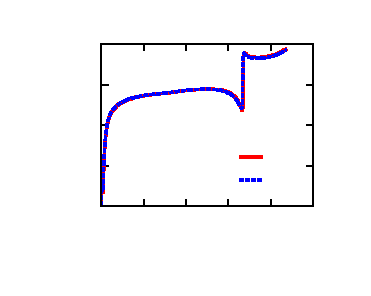
\includegraphics{ch-dynamics/conv_zst_U}}%
    \gplfronttext
  \end{picture}%
\endgroup

  \hspace{-0.40625in}
  % GNUPLOT: LaTeX picture with Postscript
\begingroup
  \makeatletter
  \providecommand\color[2][]{%
    \GenericError{(gnuplot) \space\space\space\@spaces}{%
      Package color not loaded in conjunction with
      terminal option `colourtext'%
    }{See the gnuplot documentation for explanation.%
    }{Either use 'blacktext' in gnuplot or load the package
      color.sty in LaTeX.}%
    \renewcommand\color[2][]{}%
  }%
  \providecommand\includegraphics[2][]{%
    \GenericError{(gnuplot) \space\space\space\@spaces}{%
      Package graphicx or graphics not loaded%
    }{See the gnuplot documentation for explanation.%
    }{The gnuplot epslatex terminal needs graphicx.sty or graphics.sty.}%
    \renewcommand\includegraphics[2][]{}%
  }%
  \providecommand\rotatebox[2]{#2}%
  \@ifundefined{ifGPcolor}{%
    \newif\ifGPcolor
    \GPcolortrue
  }{}%
  \@ifundefined{ifGPblacktext}{%
    \newif\ifGPblacktext
    \GPblacktexttrue
  }{}%
  % define a \g@addto@macro without @ in the name:
  \let\gplgaddtomacro\g@addto@macro
  % define empty templates for all commands taking text:
  \gdef\gplbacktext{}%
  \gdef\gplfronttext{}%
  \makeatother
  \ifGPblacktext
    % no textcolor at all
    \def\colorrgb#1{}%
    \def\colorgray#1{}%
  \else
    % gray or color?
    \ifGPcolor
      \def\colorrgb#1{\color[rgb]{#1}}%
      \def\colorgray#1{\color[gray]{#1}}%
      \expandafter\def\csname LTw\endcsname{\color{white}}%
      \expandafter\def\csname LTb\endcsname{\color{black}}%
      \expandafter\def\csname LTa\endcsname{\color{black}}%
      \expandafter\def\csname LT0\endcsname{\color[rgb]{1,0,0}}%
      \expandafter\def\csname LT1\endcsname{\color[rgb]{0,1,0}}%
      \expandafter\def\csname LT2\endcsname{\color[rgb]{0,0,1}}%
      \expandafter\def\csname LT3\endcsname{\color[rgb]{1,0,1}}%
      \expandafter\def\csname LT4\endcsname{\color[rgb]{0,1,1}}%
      \expandafter\def\csname LT5\endcsname{\color[rgb]{1,1,0}}%
      \expandafter\def\csname LT6\endcsname{\color[rgb]{0,0,0}}%
      \expandafter\def\csname LT7\endcsname{\color[rgb]{1,0.3,0}}%
      \expandafter\def\csname LT8\endcsname{\color[rgb]{0.5,0.5,0.5}}%
    \else
      % gray
      \def\colorrgb#1{\color{black}}%
      \def\colorgray#1{\color[gray]{#1}}%
      \expandafter\def\csname LTw\endcsname{\color{white}}%
      \expandafter\def\csname LTb\endcsname{\color{black}}%
      \expandafter\def\csname LTa\endcsname{\color{black}}%
      \expandafter\def\csname LT0\endcsname{\color{black}}%
      \expandafter\def\csname LT1\endcsname{\color{black}}%
      \expandafter\def\csname LT2\endcsname{\color{black}}%
      \expandafter\def\csname LT3\endcsname{\color{black}}%
      \expandafter\def\csname LT4\endcsname{\color{black}}%
      \expandafter\def\csname LT5\endcsname{\color{black}}%
      \expandafter\def\csname LT6\endcsname{\color{black}}%
      \expandafter\def\csname LT7\endcsname{\color{black}}%
      \expandafter\def\csname LT8\endcsname{\color{black}}%
    \fi
  \fi
  \setlength{\unitlength}{0.0500bp}%
  \begin{picture}(3600.00,2520.00)%
    \gplgaddtomacro\gplbacktext{%
      \csname LTb\endcsname%
      \put(1078,704){\makebox(0,0)[r]{\strut{} 600}}%
      \put(1078,1014){\makebox(0,0)[r]{\strut{} 1000}}%
      \put(1078,1325){\makebox(0,0)[r]{\strut{} 1400}}%
      \put(1078,1635){\makebox(0,0)[r]{\strut{} 1800}}%
      \put(1078,1946){\makebox(0,0)[r]{\strut{} 2200}}%
      \put(1078,2256){\makebox(0,0)[r]{\strut{} 2600}}%
      \put(1210,484){\makebox(0,0){\strut{} 0}}%
      \put(1609,484){\makebox(0,0){\strut{} 2}}%
      \put(2007,484){\makebox(0,0){\strut{} 4}}%
      \put(2406,484){\makebox(0,0){\strut{} 6}}%
      \put(2804,484){\makebox(0,0){\strut{} 8}}%
      \put(3203,484){\makebox(0,0){\strut{} 10}}%
      \put(176,1480){\rotatebox{-270}{\makebox(0,0){\strut{}\vspace{-48pt}$T$ [K]}}}%
      \put(2206,154){\makebox(0,0){\strut{}$x/D$}}%
      \put(1459,2023){\makebox(0,0)[l]{\strut{}Nominal}}%
      \put(1459,1790){\makebox(0,0)[l]{\strut{}Coarser}}%
    }%
    \gplgaddtomacro\gplfronttext{%
      \csname LTb\endcsname%
      \put(1871,2037){\makebox(0,0)[r]{\strut{} }}%
      \csname LTb\endcsname%
      \put(1871,1817){\makebox(0,0)[r]{\strut{} }}%
    }%
    \gplbacktext
    \put(0,0){
\includegraphics{conv_zst_T}}%
    \gplfronttext
  \end{picture}%
\endgroup

  \hspace{-0.40625in}
  % GNUPLOT: LaTeX picture with Postscript
\begingroup
  \makeatletter
  \providecommand\color[2][]{%
    \GenericError{(gnuplot) \space\space\space\@spaces}{%
      Package color not loaded in conjunction with
      terminal option `colourtext'%
    }{See the gnuplot documentation for explanation.%
    }{Either use 'blacktext' in gnuplot or load the package
      color.sty in LaTeX.}%
    \renewcommand\color[2][]{}%
  }%
  \providecommand\includegraphics[2][]{%
    \GenericError{(gnuplot) \space\space\space\@spaces}{%
      Package graphicx or graphics not loaded%
    }{See the gnuplot documentation for explanation.%
    }{The gnuplot epslatex terminal needs graphicx.sty or graphics.sty.}%
    \renewcommand\includegraphics[2][]{}%
  }%
  \providecommand\rotatebox[2]{#2}%
  \@ifundefined{ifGPcolor}{%
    \newif\ifGPcolor
    \GPcolortrue
  }{}%
  \@ifundefined{ifGPblacktext}{%
    \newif\ifGPblacktext
    \GPblacktexttrue
  }{}%
  % define a \g@addto@macro without @ in the name:
  \let\gplgaddtomacro\g@addto@macro
  % define empty templates for all commands taking text:
  \gdef\gplbacktext{}%
  \gdef\gplfronttext{}%
  \makeatother
  \ifGPblacktext
    % no textcolor at all
    \def\colorrgb#1{}%
    \def\colorgray#1{}%
  \else
    % gray or color?
    \ifGPcolor
      \def\colorrgb#1{\color[rgb]{#1}}%
      \def\colorgray#1{\color[gray]{#1}}%
      \expandafter\def\csname LTw\endcsname{\color{white}}%
      \expandafter\def\csname LTb\endcsname{\color{black}}%
      \expandafter\def\csname LTa\endcsname{\color{black}}%
      \expandafter\def\csname LT0\endcsname{\color[rgb]{1,0,0}}%
      \expandafter\def\csname LT1\endcsname{\color[rgb]{0,1,0}}%
      \expandafter\def\csname LT2\endcsname{\color[rgb]{0,0,1}}%
      \expandafter\def\csname LT3\endcsname{\color[rgb]{1,0,1}}%
      \expandafter\def\csname LT4\endcsname{\color[rgb]{0,1,1}}%
      \expandafter\def\csname LT5\endcsname{\color[rgb]{1,1,0}}%
      \expandafter\def\csname LT6\endcsname{\color[rgb]{0,0,0}}%
      \expandafter\def\csname LT7\endcsname{\color[rgb]{1,0.3,0}}%
      \expandafter\def\csname LT8\endcsname{\color[rgb]{0.5,0.5,0.5}}%
    \else
      % gray
      \def\colorrgb#1{\color{black}}%
      \def\colorgray#1{\color[gray]{#1}}%
      \expandafter\def\csname LTw\endcsname{\color{white}}%
      \expandafter\def\csname LTb\endcsname{\color{black}}%
      \expandafter\def\csname LTa\endcsname{\color{black}}%
      \expandafter\def\csname LT0\endcsname{\color{black}}%
      \expandafter\def\csname LT1\endcsname{\color{black}}%
      \expandafter\def\csname LT2\endcsname{\color{black}}%
      \expandafter\def\csname LT3\endcsname{\color{black}}%
      \expandafter\def\csname LT4\endcsname{\color{black}}%
      \expandafter\def\csname LT5\endcsname{\color{black}}%
      \expandafter\def\csname LT6\endcsname{\color{black}}%
      \expandafter\def\csname LT7\endcsname{\color{black}}%
      \expandafter\def\csname LT8\endcsname{\color{black}}%
    \fi
  \fi
  \setlength{\unitlength}{0.0500bp}%
  \begin{picture}(3744.00,2520.00)%
    \gplgaddtomacro\gplbacktext{%
      \csname LTb\endcsname%
      \put(1210,704){\makebox(0,0)[r]{\strut{} 0}}%
      \put(1210,1014){\makebox(0,0)[r]{\strut{} 0.002}}%
      \put(1210,1325){\makebox(0,0)[r]{\strut{} 0.004}}%
      \put(1210,1635){\makebox(0,0)[r]{\strut{} 0.006}}%
      \put(1210,1946){\makebox(0,0)[r]{\strut{} 0.008}}%
      \put(1210,2256){\makebox(0,0)[r]{\strut{} 0.01}}%
      \put(1342,484){\makebox(0,0){\strut{} 0}}%
      \put(1743,484){\makebox(0,0){\strut{} 2}}%
      \put(2144,484){\makebox(0,0){\strut{} 4}}%
      \put(2545,484){\makebox(0,0){\strut{} 6}}%
      \put(2946,484){\makebox(0,0){\strut{} 8}}%
      \put(3347,484){\makebox(0,0){\strut{} 10}}%
      \put(176,1480){\rotatebox{-270}{\makebox(0,0){\strut{}\vspace{-52pt}$Y_{\rm H_2O_2}$}}}%
      \put(2344,154){\makebox(0,0){\strut{}$x/D$}}%
      \put(1593,2023){\makebox(0,0)[l]{\strut{}Nominal}}%
      \put(1593,1790){\makebox(0,0)[l]{\strut{}Coarser}}%
    }%
    \gplgaddtomacro\gplfronttext{%
      \csname LTb\endcsname%
      \put(2035,2022){\makebox(0,0)[r]{\strut{} }}%
      \csname LTb\endcsname%
      \put(2035,1802){\makebox(0,0)[r]{\strut{} }}%
    }%
    \gplbacktext
    \put(0,0){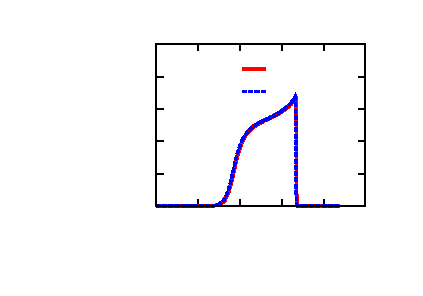
\includegraphics{conv_zst_H2O2}}%
    \gplfronttext
  \end{picture}%
\endgroup

%  \vspace{-0.1875in}
  \normalsize
  \caption{Velocity, temperature, and H$_2$O$_2$ profiles along $Z_{\rm st}$ on the nominal and two times coarser meshes.}
  \label{fig:convergence}
\end{figure}

\section{Computational Method and Diagnostic Tool}
\subsection{Chemical Explosive Mode Analysis}

The numerical diagnostic tool, Chemical Explosive Mode Analysis (CEMA) was developed by Lu and co-workers~\cite{lu10,ruiqin12} and was adopted in the present study to identify the controlling chemistry in complex flows.  Briefly, the eigenvalues of the Jacobian matrix of the chemical source term based on the local species concentrations and temperature is evaluated and determined as the chemical modes.  The largest positive eigenvalue, which is defined as the chemical explosive mode, describes the rate of the system runaway.  The projection of a reaction and radical on the explosive mode are defined as the explosion participation index and radical explosion pointer, respectively, to account for their contribution to the explosive mode.  In the present study, species concentrations and temperatures were sampled at certain locations of interest from the NGA simulation and processed with CEMA.  Based on the explosive mode and participation index, species and reactions having the most influence on ignition and flame structure can be readily identified.

\subsection{Lagrangian Flamelet Model} \label{sec:LFM}

To the role of autoignition for the current flow configuration, a direct comparison with the homogeneous counterpart for a Lagrangian flow particle is insufficient, since the transport terms both along and perpendicular to the mixture fraction gradient is neglected in the homogeneous case.  On one hand, the species stratification along mixture fraction gradient can significantly modify the ignition characteristics, especially for fuels with NTC chemistry~\cite{law12,deng14}.  On the other hand, the flame propagation along the mixture fraction iso-contour can also influence the autoignition front through thermal and radical back diffusion.  To reveal these effects, an unsteady nonpremixed flamelet, corresponding to the mixing layer,  was computed to capture the stratification effects along the mixture fraction gradient, characterized by the dissipation rate.  Therefore, the comparison between the one-dimensional unsteady flamelet and the two-dimensional coflow simulation reveals the role of the transport processes along mixture fraction iso-contours, more specificly, the interaction between the autoignition front and the flame structure.  

The unsteady flamelet model developed by Pitsch \emph{et al.}~\cite{pitsch98a}, which is called the Lagrangian Flamelet Model (LFM), was adopted to investigate the evolution of the autoignitive mixing layer.  Due to mixing processes, the dissipation rate $\chi$, which can influence the flamelet solution significantly, decreases along the stream axis.  Therefore, this dissipation rate variation should be considered when simulating a flamelet that is transported downstream.  

In the present study, the unsteady flamelet was simulated with the FlameMaster code~\cite{flamemaster}, and the dissipation rate was specified as a function of the flamelet time.  The flamelet time was computed from the NGA simulation result, along the stoichiometric mixture fraction $Z_{\rm st}$ iso-contour, through Eqn.~\ref{eqn:t}. 
 \begin{equation} \label{eqn:t}
t = \int ^{x}_{0} \frac{1}{(u + u_Z)(x')|(Z=Z_{\rm st})} dx'.
\end{equation}
This formulation is otherwise the same as in Pitsch \emph {et al.}~\cite{pitsch98a}, except that in addition to the axial component of the fluid convection velocity $u$, the axial component of the mixture fraction iso-contour propagation speed relative to the fluid convection $u_Z$ is also taken into account.

The expression for the constant property scalar iso-surface velocity relative to the local fluid motion was derived by Pope~\cite{pope88(S.B. Pope, Int.J. Eng. Sci. 26 (1988) 445-469)}, and the current work adopted the formulation derived by Lignell \emph {et al.}~\cite{lignell07(D.O. Lignell Combustion and Flames 151 (2007) 2-28)} for variable properties, as
\begin{equation}
\mathbf{u_Z} = -\frac{\nabla \cdot (\rho D_Z \nabla Z) }{\rho |\nabla Z|} \mathbf{n},
\end{equation}  
where $D_Z$ is the mixture fraction diffusivity and $\rho$ is the density.  The normal vector \textbf{n} indicates the direction of this diffusion induced relative velocity, defined by  
\begin{equation}
\mathbf{n} = \frac{\nabla Z}{|\nabla Z|}.
\end{equation}

The dissipation rate along the $Z_{\rm st} = 0.1005$ iso-contour obtained from the NGA simulation was then correlated with this flamelet time and provided as the input for the FlameMaster calculation.  The dissipation rates at other mixture fractions were computed by FlameMaster, following~\cite{petersbook}
\begin{equation} \label{eqn:Zref}
\chi{(Z)} = \chi{(Z_{\rm st})} \frac{\exp{(-2[{\rm erfc}^{-1}(2Z)]^2)}}{\exp{(-2[{\rm erfc}^{-1}(2Z_{\rm st})]^2)}}.
\end{equation}

To validate this formulation in the current configuration, the dissipation rates along different mixture fraction iso-contours were sampled from the NGA simulation, normalized using Eqn.~\ref{eqn:Zref}, and compared with the sampling along the $Z_{\rm st}$ iso-contour.  As shown in Fig.~\ref{fig:Zref}, the normalized dissipation rates at different mixture fractions all collapse to the value at $Z_{\rm st}$.  Therefore, only the dissipation rate samplings along the $Z_{\rm st}$ iso-contour were needed to perform the unsteady flamelet calculation.

To account for the differential diffusion, species Lewis numbers for LFM  were specified the same as in the NGA simulation.  The governing equations for species and temperature follow Eqn. $24$ and $25$ in Pitsch and Peters~\cite{pitsch98b}.


\begin{figure}
  \centering
  \scriptsize
  % GNUPLOT: LaTeX picture with Postscript
\begingroup
  \makeatletter
  \providecommand\color[2][]{%
    \GenericError{(gnuplot) \space\space\space\@spaces}{%
      Package color not loaded in conjunction with
      terminal option `colourtext'%
    }{See the gnuplot documentation for explanation.%
    }{Either use 'blacktext' in gnuplot or load the package
      color.sty in LaTeX.}%
    \renewcommand\color[2][]{}%
  }%
  \providecommand\includegraphics[2][]{%
    \GenericError{(gnuplot) \space\space\space\@spaces}{%
      Package graphicx or graphics not loaded%
    }{See the gnuplot documentation for explanation.%
    }{The gnuplot epslatex terminal needs graphicx.sty or graphics.sty.}%
    \renewcommand\includegraphics[2][]{}%
  }%
  \providecommand\rotatebox[2]{#2}%
  \@ifundefined{ifGPcolor}{%
    \newif\ifGPcolor
    \GPcolortrue
  }{}%
  \@ifundefined{ifGPblacktext}{%
    \newif\ifGPblacktext
    \GPblacktexttrue
  }{}%
  % define a \g@addto@macro without @ in the name:
  \let\gplgaddtomacro\g@addto@macro
  % define empty templates for all commands taking text:
  \gdef\gplbacktext{}%
  \gdef\gplfronttext{}%
  \makeatother
  \ifGPblacktext
    % no textcolor at all
    \def\colorrgb#1{}%
    \def\colorgray#1{}%
  \else
    % gray or color?
    \ifGPcolor
      \def\colorrgb#1{\color[rgb]{#1}}%
      \def\colorgray#1{\color[gray]{#1}}%
      \expandafter\def\csname LTw\endcsname{\color{white}}%
      \expandafter\def\csname LTb\endcsname{\color{black}}%
      \expandafter\def\csname LTa\endcsname{\color{black}}%
      \expandafter\def\csname LT0\endcsname{\color[rgb]{1,0,0}}%
      \expandafter\def\csname LT1\endcsname{\color[rgb]{0,1,0}}%
      \expandafter\def\csname LT2\endcsname{\color[rgb]{0,0,1}}%
      \expandafter\def\csname LT3\endcsname{\color[rgb]{1,0,1}}%
      \expandafter\def\csname LT4\endcsname{\color[rgb]{0,1,1}}%
      \expandafter\def\csname LT5\endcsname{\color[rgb]{1,1,0}}%
      \expandafter\def\csname LT6\endcsname{\color[rgb]{0,0,0}}%
      \expandafter\def\csname LT7\endcsname{\color[rgb]{1,0.3,0}}%
      \expandafter\def\csname LT8\endcsname{\color[rgb]{0.5,0.5,0.5}}%
    \else
      % gray
      \def\colorrgb#1{\color{black}}%
      \def\colorgray#1{\color[gray]{#1}}%
      \expandafter\def\csname LTw\endcsname{\color{white}}%
      \expandafter\def\csname LTb\endcsname{\color{black}}%
      \expandafter\def\csname LTa\endcsname{\color{black}}%
      \expandafter\def\csname LT0\endcsname{\color{black}}%
      \expandafter\def\csname LT1\endcsname{\color{black}}%
      \expandafter\def\csname LT2\endcsname{\color{black}}%
      \expandafter\def\csname LT3\endcsname{\color{black}}%
      \expandafter\def\csname LT4\endcsname{\color{black}}%
      \expandafter\def\csname LT5\endcsname{\color{black}}%
      \expandafter\def\csname LT6\endcsname{\color{black}}%
      \expandafter\def\csname LT7\endcsname{\color{black}}%
      \expandafter\def\csname LT8\endcsname{\color{black}}%
    \fi
  \fi
  \setlength{\unitlength}{0.0500bp}%
  \begin{picture}(7200.00,5040.00)%
    \gplgaddtomacro\gplbacktext{%
      \csname LTb\endcsname%
      \put(946,704){\makebox(0,0)[r]{\strut{} 0}}%
      \put(946,1383){\makebox(0,0)[r]{\strut{} 50}}%
      \put(946,2061){\makebox(0,0)[r]{\strut{} 100}}%
      \put(946,2740){\makebox(0,0)[r]{\strut{} 150}}%
      \put(946,3418){\makebox(0,0)[r]{\strut{} 200}}%
      \put(946,4097){\makebox(0,0)[r]{\strut{} 250}}%
      \put(946,4775){\makebox(0,0)[r]{\strut{} 300}}%
      \put(1078,484){\makebox(0,0){\strut{} 0}}%
      \put(1841,484){\makebox(0,0){\strut{} 0.2}}%
      \put(2605,484){\makebox(0,0){\strut{} 0.4}}%
      \put(3368,484){\makebox(0,0){\strut{} 0.6}}%
      \put(4131,484){\makebox(0,0){\strut{} 0.8}}%
      \put(4895,484){\makebox(0,0){\strut{} 1}}%
      \put(5658,484){\makebox(0,0){\strut{} 1.2}}%
      \put(6421,484){\makebox(0,0){\strut{} 1.4}}%
      \put(176,2739){\rotatebox{-270}{\makebox(0,0){\strut{}\vspace{-28pt}$\frac{\chi(Z)}{f(Z,Z_{\rm st})}$ [1/s]}}}%
      \put(3940,154){\makebox(0,0){\strut{}Time [ms]}}%
    }%
    \gplgaddtomacro\gplfronttext{%
      \csname LTb\endcsname%
      \put(5816,4602){\makebox(0,0)[r]{\strut{}$Z = Z_{\rm st}$}}%
      \csname LTb\endcsname%
      \put(5816,4382){\makebox(0,0)[r]{\strut{}$Z = 0.2$}}%
      \csname LTb\endcsname%
      \put(5816,4162){\makebox(0,0)[r]{\strut{}$Z = 0.4$}}%
      \csname LTb\endcsname%
      \put(5816,3942){\makebox(0,0)[r]{\strut{}$Z = 0.6$}}%
    }%
    \gplbacktext
    \put(0,0){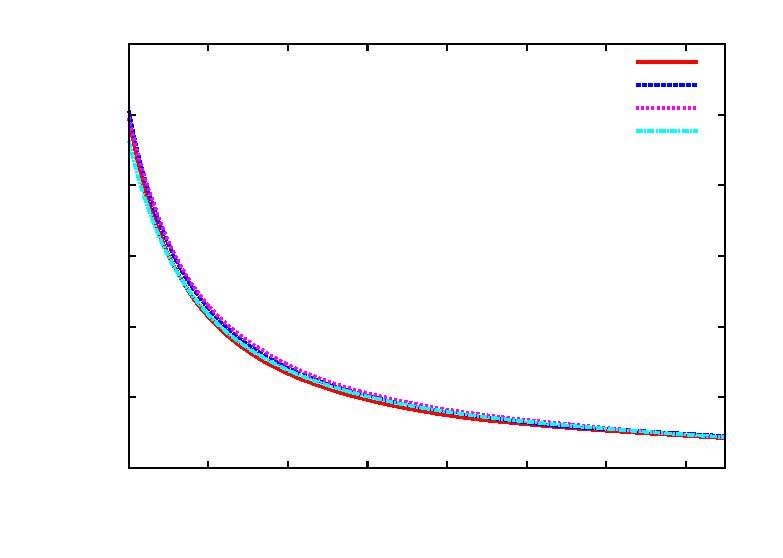
\includegraphics{Zref}}%
    \gplfronttext
  \end{picture}%
\endgroup

  \normalsize
  \caption{The comparison between the sampled and converted $\chi_{\rm st}$ based on NGA simulation at $800$ K and Eqn.~\ref{eqn:Zref}.}
  \label{fig:Zref}
\end{figure}

\section{Results and Discussion} 

\begin{figure}[t]
  \centering
  \scriptsize
  \vspace{-0.1in}
  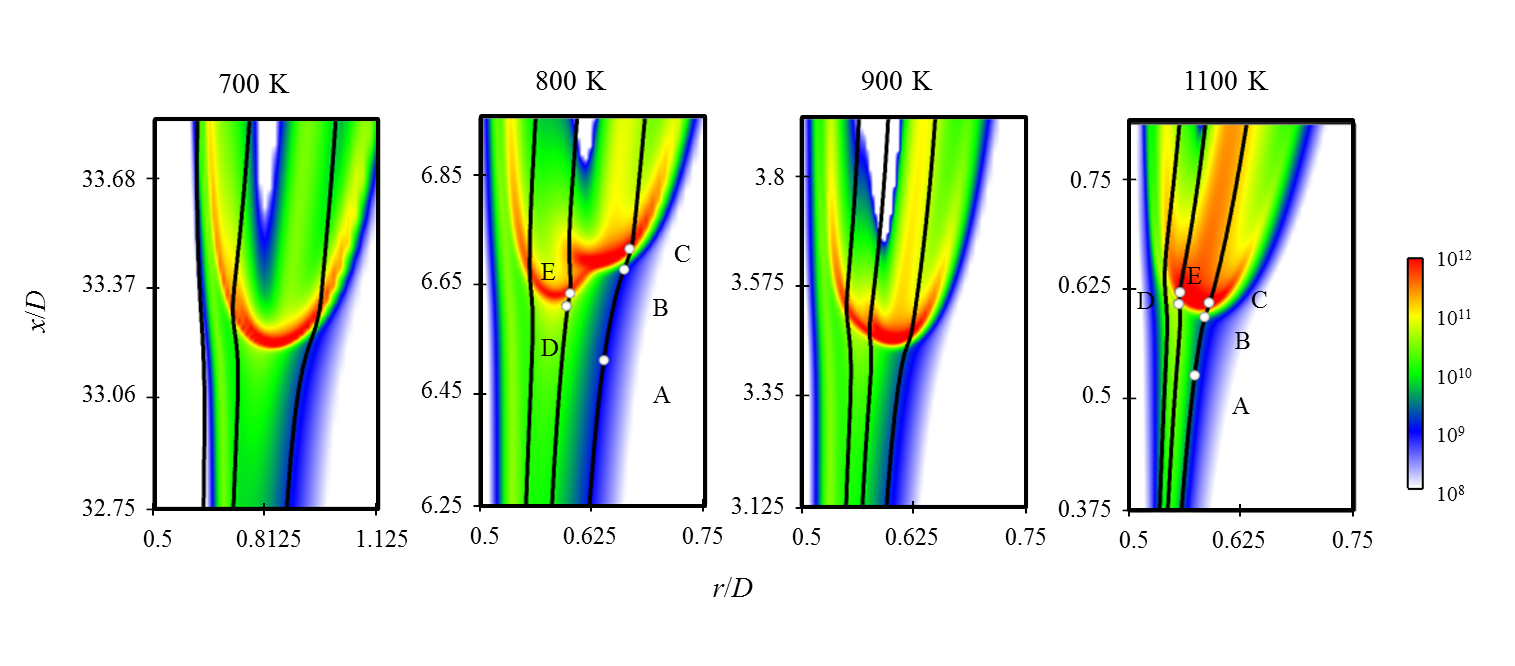
\includegraphics[width=1.0\textwidth]{HRR.png}
  \normalsize
  \vspace{-0.1in}
  \caption{Heat release rate [Jm$^{-3}$s$^{-1}$] profiles.  The iso-furfaces of $Z_{\rm st}$, $Z = 0.2$, and $Z = 0.3$ are outlined from left to right in solid lines, respectively.  The sampling points at $800$ and $1100$ K are marked along the iso-contours for CEMA.}
  \label{fig:HRR}
\end{figure}

To visualize the flame structure, the heat release rates for the $700$, $800$, $900$, and $1100$ K cases were shown in Fig.~\ref{fig:HRR}.  Qualitatively, the most upstream point on the largest heat release contour, colored by red, was estimated as the stabilization point.  At $700$ K, a tribrachial thermal structure is observed, and the stabilization point locates around $Z = 0.15$, which is richer than the triple point.  Moreover, compared to the classical triple flame structure, the middle heat release rate branch, corresponding to the nonpremixed flame, is significantly weaker than the other two premixed branches.  At $800$ K, the stabilization point does not locate on the triple flame structure any more.  Instead, it locates near $Z = 0.23$ and connects two trailing heat release branches, where a triple flame structure attaches to the leaner branch.  As the air boundary temperature increases to $900$ K, the holding front, corresponding to the $800$ K case, becomes a trailing branch that attaches to the rich premixed branch of the triple flame structure, and the stabilization point shifts to $Z = 0.14$.  A further increase in the boundary temperature results in a structure that is very similar to the classical triple flame, except for the fact that there is also heat release from the upstream ahead of the stabilization point at $Z = 0.13$.  Some of the multibrachial structures were also observed by Krisman \emph{et al.}~\cite{krisman14}, and it was concluded in that reference that the autoignition chemistry could affect the flame structure and the stabilization mechanism.  

To first qualitatively demonstrate the chemical structure of the flame, selected species profiles were examined, shown in~\Cref{fig:OH,fig:RO2,fig:HO2,fig:H2O2}.  The methoxymethylperoxy radical (CH$_3$OCH$_2$O$_2$) and hydroxyl radical (OH) were chosen, as indicators of low and high temperature chemistry, repectively.  The hydroperoxyl radical (HO$_2$) and hydrogen peroxide (H$_2$O$_2$) were chosen, as they form in the preheat zone of a flame or before autoignition, but quickly vanish in the post flame zone or after ignition~\cite{yoo09}.  

The low temperature chemistry, which is indicated by the CH$_3$OCH$_2$O$_2$ radical, is found to be important at richer mixture fractions, where the temperature is lower.  On the other hand, in the flame region, OH radical peaks where corresponds to the triple flame structure.  For the $800$ and $900$ K cases, another OH local maxima appears at richer mixture fractions, right downstream where the CH$_3$OCH$_2$O$_2$ radical and H$_2$O$_2$ disappear, indicating autoignition.  For the $700$ to $900$ K cases, the locations of the peaking HO$_2$ mass fraction and heat release rate contours outline the flame front and the reactive mixture at the rich mixture fractions.  It is interesting that, for these three cases, the upstream region ahead of the flame front also has relatively high HO$_2$ mass fractions.  On the contrary, HO$_2$ radical accumulation is not observed ahead of the flame at $1100$ K.  Moreover, the H$_2$O$_2$ radical profiles show more pronounced difference between the $1100$ K case and three lower boundary temperature cases: H$_2$O$_2$ radical accumulates from upstream for the lower boundary temperature cases, until it decomposes at the flame region, while for the $1100$ K case, H$_2$O$_2$ accumulation is an order of magnitude lower, due to the reduced residence time from the nozzle exits to the flame base.

\begin{figure}[t]
  \centering
  \scriptsize
  \vspace{-0.1in}
  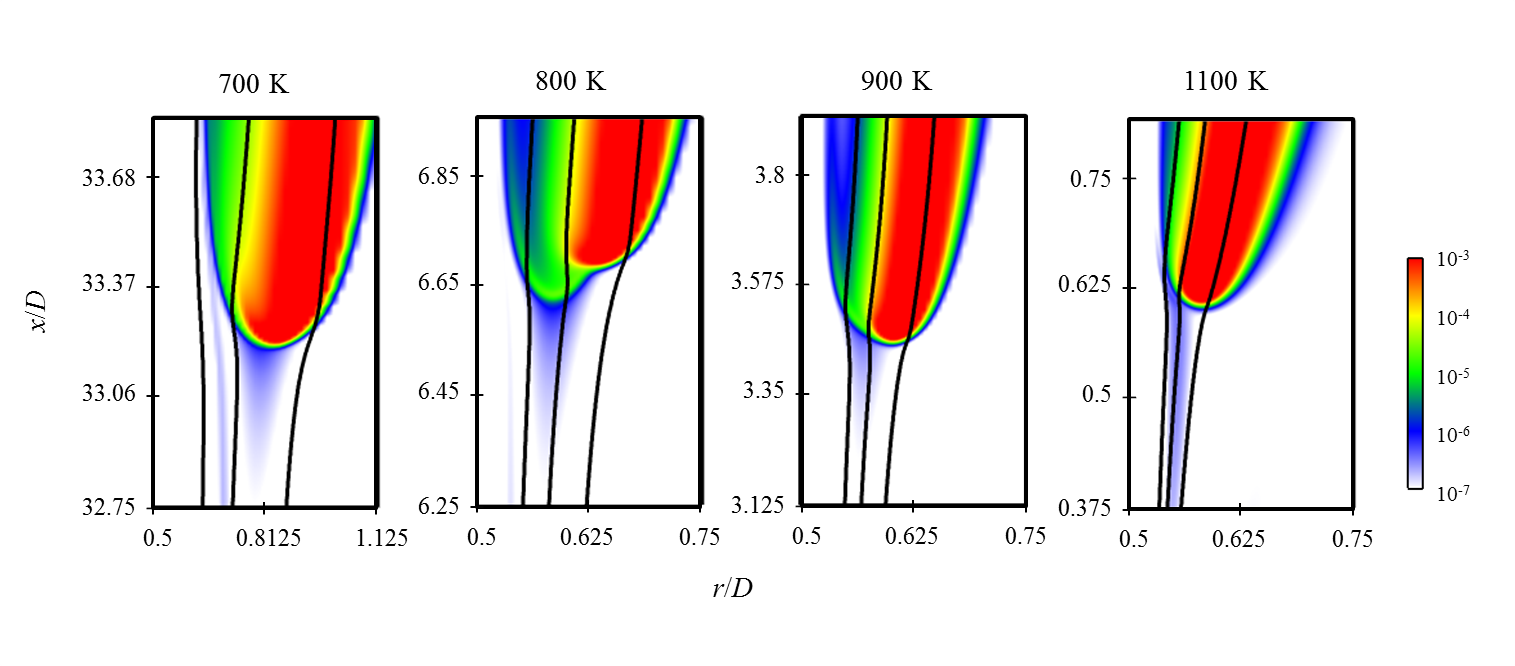
\includegraphics[width=1.0\textwidth]{OH.png}
  \normalsize
  \vspace{-0.1in}
  \caption{Hydroxyl radical mass fraction profiles.  The iso-furfaces of $Z_{\rm st}$, $Z = 0.2$, and $Z = 0.3$ are outlined from left to right in solid lines, respectively.}
  \label{fig:OH}
\end{figure}

\begin{figure}[t]
  \centering
  \scriptsize
  \vspace{-0.1in}
  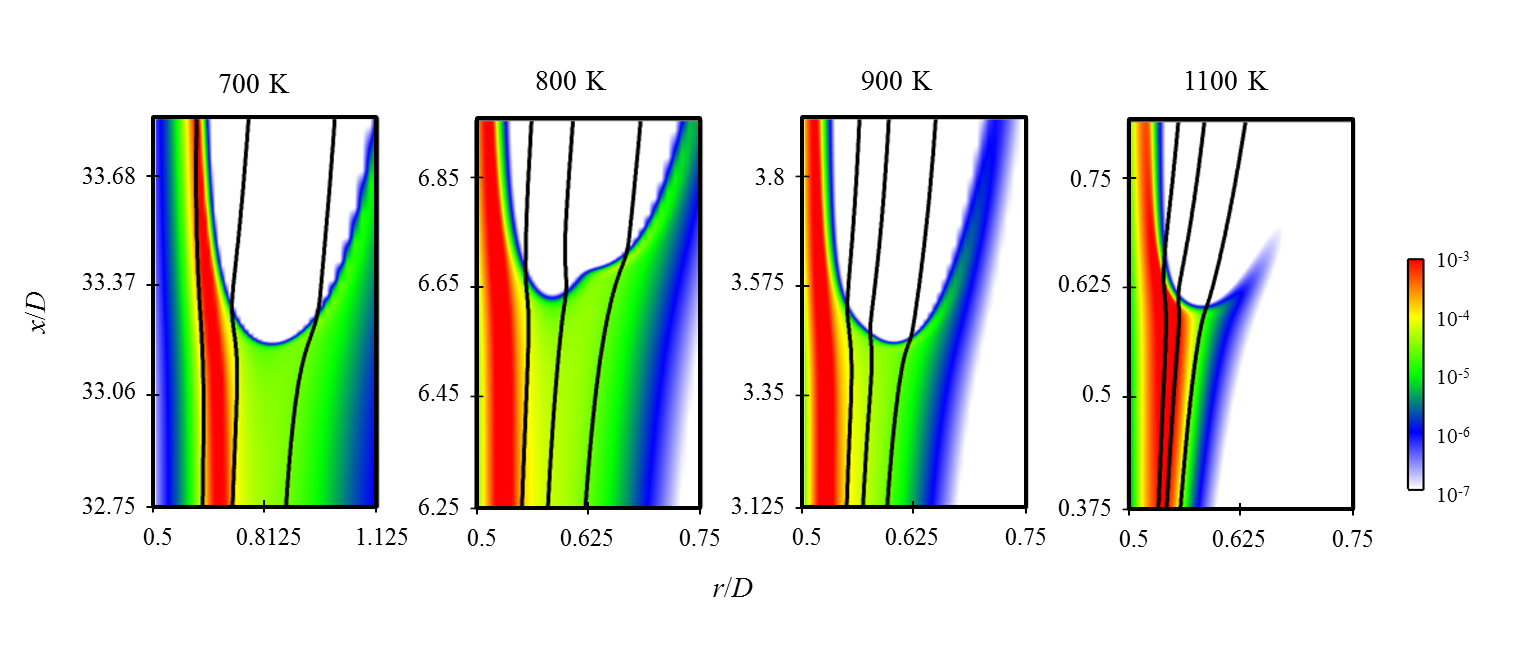
\includegraphics[width=1.0\textwidth]{RO2.png}
  \normalsize
  \vspace{-0.1in}
  \caption{Methoxymethylperoxy radical mass fraction profiles.  The iso-furfaces of $Z_{\rm st}$, $Z = 0.2$, and $Z = 0.3$ are outlined from left to right in solid lines, respectively.}
  \label{fig:RO2}
\end{figure}

\begin{figure}[t]
  \centering
  \scriptsize
  \vspace{-0.1in}
  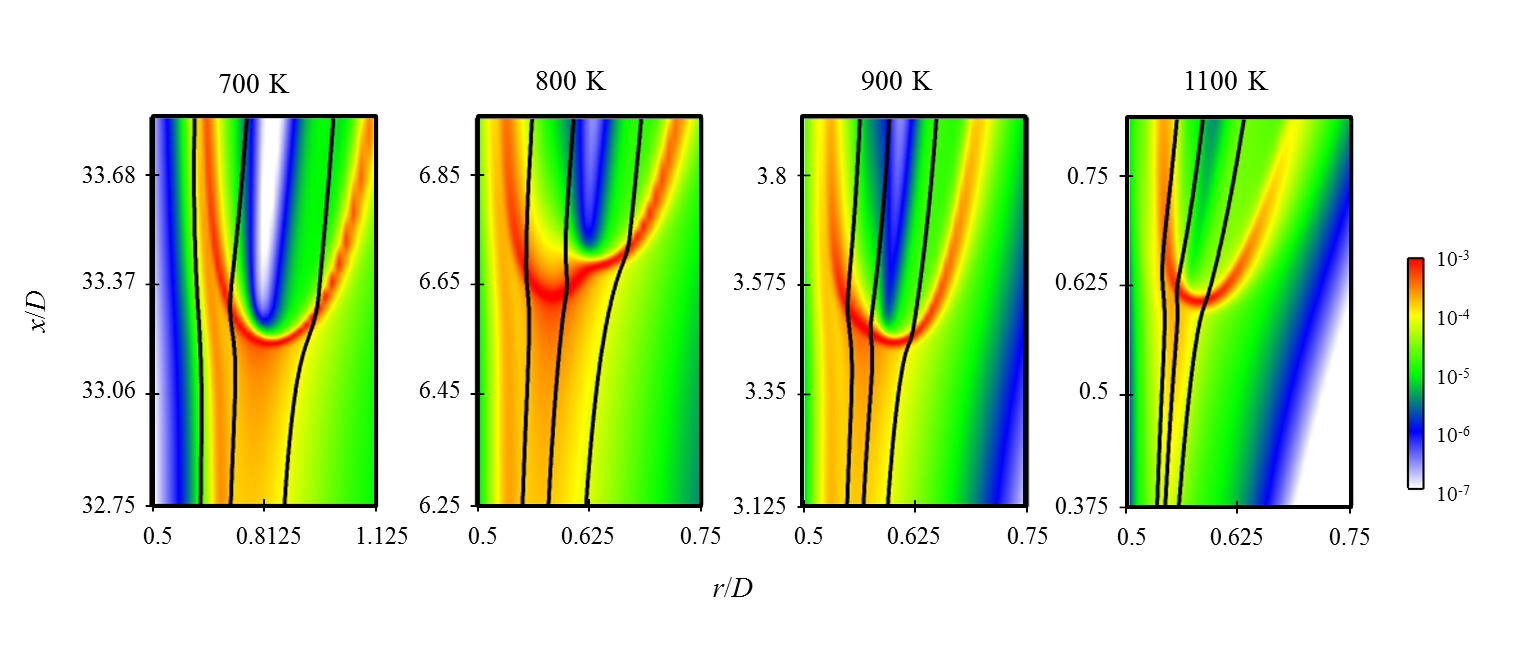
\includegraphics[width=1.0\textwidth]{HO2.png}
  \normalsize
  \vspace{-0.1in}
  \caption{Hydroperoxyl radical mass fraction profiles.  The iso-furfaces of $Z_{\rm st}$, $Z = 0.2$, and $Z = 0.3$ are outlined from left to right in solid lines, respectively.}
  \label{fig:HO2}
\end{figure}

\begin{figure}[t]
  \centering
  \scriptsize
  \vspace{-0.1in}
  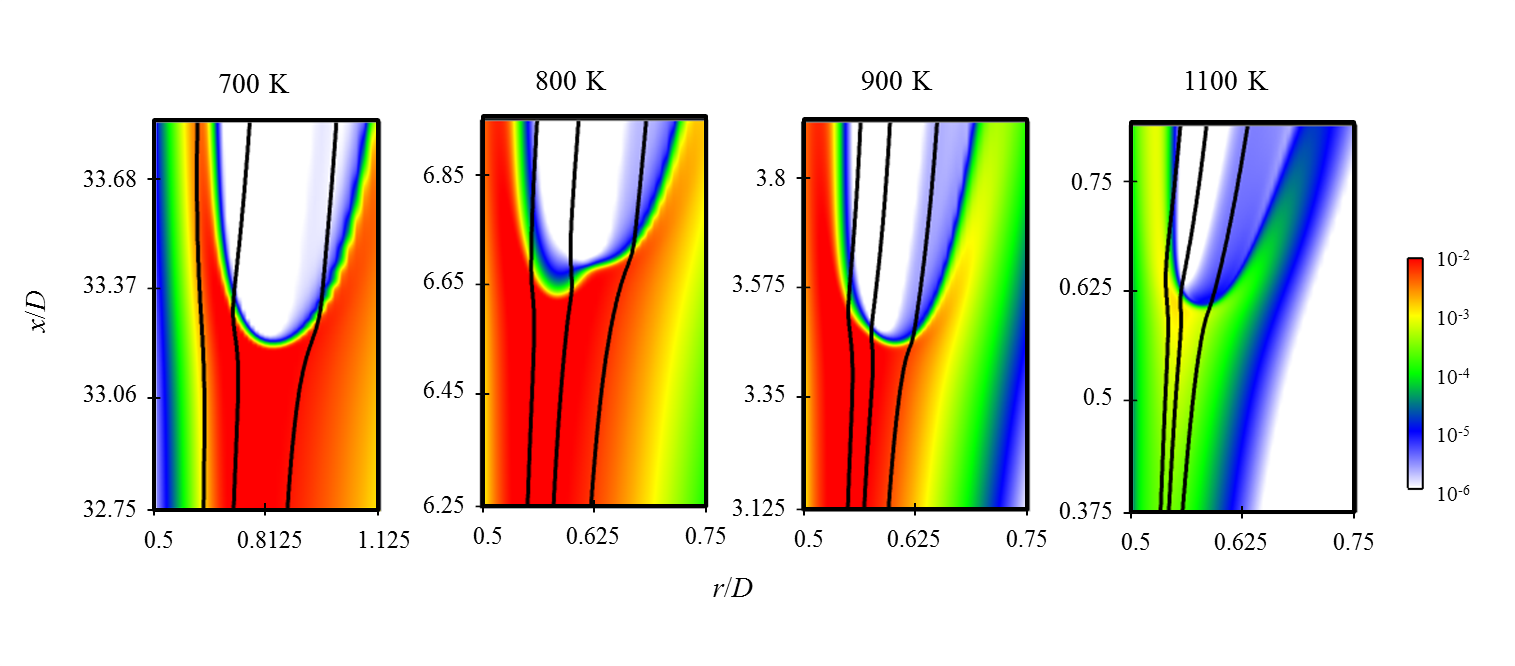
\includegraphics[width=1.0\textwidth]{H2O2.png}
  \normalsize
  \vspace{-0.1in}
  \caption{Hydrogen peroxide mass fraction profiles.  The iso-furfaces of $Z_{\rm st}$, $Z = 0.2$, and $Z = 0.3$ are outlined from left to right in solid lines, respectively.}
  \label{fig:H2O2}
\end{figure}

Besides the analysis based on selected species profiles, Chemical Explosive Mode Analysis was conducted, as it can determine not only the explosive nature of the local mixture, but also the contribution from each chemical reaction and relative importance of radicals.  Therefore, the dominating reactions at characteristic locations, such as those upstream and near the flame base can be identified.  For each case, the local species concentrations and temperature were sampled along the $Z_{\rm st}$, $Z = 0.2$, and $Z = 0.3$ iso-contours and process by CEMA to demonstrate the evolution of the dominating reactions.

For the three lower coflow temperature cases, similar chemical patterns were found.  Upstream the flame front, the eigenvalues of the chemical modes are positive, indicating that the mixtures have the potential to explode, while after the flame front, the eigenvalues become negative, meaning that the mixtures are composed of burned products.  Following the $Z_{\rm st}$ iso-contour, the hydrogen peroxide chain branching reaction (H$_2$O$_2$ + M $\Longleftrightarrow$ OH + OH + M) is the reaction that has the largest projection on the explosive mode, showing the dominating role of autoignition chain branching.  The characteristic DME low temperature chemistry is also important upstream the flame, where the methoxymethylperoxy radical formation (CH$_3$OCH$_2$ + O$_2$ $\Longleftrightarrow$ CH$_3$OCH$_2$O$_2$) and the isomerization (CH$_3$OCH$_2$O$_2$ $\Longleftrightarrow$ CH$_2$OCH$_2$O$_2$H) reaction promotes the explosion, while the $\beta$-scission reaction (CH$_2$OCH$_2$O$_2$H $\Longleftrightarrow$ OH + CH$_2$O + CH$_2$O) retards the explosion.  Approaching the flame front, the H radical recombination reaction (H + O$_2$ + M $\Longleftrightarrow$ HO$_2$) becomes important for the $800$ and $900$ K cases, due to the fact that the H radical generated at the reaction zone diffuses upstream and undergoes the three-body recombination reactions under the high pressure low temperature condition.  Further downstream where the heat release rate peaks, the hydrogen branching reaction (H + O$_2$ $\Longleftrightarrow$ O + OH) becomes the most important chain branching reaction, indicating that the combustion mode alters from autoignition to flame propagation.  CEMA was conducted along other mixture fraction iso-contours, showing similar chemical mode evolution trends compared to the $Z_{\rm st}$, except the fact that the H radical recombination reaction is less important ahead of the rich heat release front in $800$ and $900$ K case.

On the contrary, although the low temperature chemistry is still important for the $1100$ K case, the hydrogen peroxide chain branching reaction is not, while the hydrogen chain branching reaction is present at the reaction zone.  As the hydrogen peroxide reaction is the crucial chain branching reaction to the autoignition process, it is thus proposed that the $1100$ K case is less affected by the autoignition chemistry than the other lower boundary temperature cases.  The above CEMA results were summarized in Fig.~\ref{fig:CEMA}, where three representative locations along the $Z_{\rm st}$ iso-contour approaching the flame front and the location ahead of the reaction front at $Z = 0.2$ were sampled.  The $800$ K case results were shown on the left, while the results for the $1100$ K case were on the right for comparison.   

\begin{figure}
  \centering
  \scriptsize
  % GNUPLOT: LaTeX picture with Postscript
\begingroup
  \makeatletter
  \providecommand\color[2][]{%
    \GenericError{(gnuplot) \space\space\space\@spaces}{%
      Package color not loaded in conjunction with
      terminal option `colourtext'%
    }{See the gnuplot documentation for explanation.%
    }{Either use 'blacktext' in gnuplot or load the package
      color.sty in LaTeX.}%
    \renewcommand\color[2][]{}%
  }%
  \providecommand\includegraphics[2][]{%
    \GenericError{(gnuplot) \space\space\space\@spaces}{%
      Package graphicx or graphics not loaded%
    }{See the gnuplot documentation for explanation.%
    }{The gnuplot epslatex terminal needs graphicx.sty or graphics.sty.}%
    \renewcommand\includegraphics[2][]{}%
  }%
  \providecommand\rotatebox[2]{#2}%
  \@ifundefined{ifGPcolor}{%
    \newif\ifGPcolor
    \GPcolortrue
  }{}%
  \@ifundefined{ifGPblacktext}{%
    \newif\ifGPblacktext
    \GPblacktexttrue
  }{}%
  % define a \g@addto@macro without @ in the name:
  \let\gplgaddtomacro\g@addto@macro
  % define empty templates for all commands taking text:
  \gdef\gplbacktext{}%
  \gdef\gplfronttext{}%
  \makeatother
  \ifGPblacktext
    % no textcolor at all
    \def\colorrgb#1{}%
    \def\colorgray#1{}%
  \else
    % gray or color?
    \ifGPcolor
      \def\colorrgb#1{\color[rgb]{#1}}%
      \def\colorgray#1{\color[gray]{#1}}%
      \expandafter\def\csname LTw\endcsname{\color{white}}%
      \expandafter\def\csname LTb\endcsname{\color{black}}%
      \expandafter\def\csname LTa\endcsname{\color{black}}%
      \expandafter\def\csname LT0\endcsname{\color[rgb]{1,0,0}}%
      \expandafter\def\csname LT1\endcsname{\color[rgb]{0,1,0}}%
      \expandafter\def\csname LT2\endcsname{\color[rgb]{0,0,1}}%
      \expandafter\def\csname LT3\endcsname{\color[rgb]{1,0,1}}%
      \expandafter\def\csname LT4\endcsname{\color[rgb]{0,1,1}}%
      \expandafter\def\csname LT5\endcsname{\color[rgb]{1,1,0}}%
      \expandafter\def\csname LT6\endcsname{\color[rgb]{0,0,0}}%
      \expandafter\def\csname LT7\endcsname{\color[rgb]{1,0.3,0}}%
      \expandafter\def\csname LT8\endcsname{\color[rgb]{0.5,0.5,0.5}}%
    \else
      % gray
      \def\colorrgb#1{\color{black}}%
      \def\colorgray#1{\color[gray]{#1}}%
      \expandafter\def\csname LTw\endcsname{\color{white}}%
      \expandafter\def\csname LTb\endcsname{\color{black}}%
      \expandafter\def\csname LTa\endcsname{\color{black}}%
      \expandafter\def\csname LT0\endcsname{\color{black}}%
      \expandafter\def\csname LT1\endcsname{\color{black}}%
      \expandafter\def\csname LT2\endcsname{\color{black}}%
      \expandafter\def\csname LT3\endcsname{\color{black}}%
      \expandafter\def\csname LT4\endcsname{\color{black}}%
      \expandafter\def\csname LT5\endcsname{\color{black}}%
      \expandafter\def\csname LT6\endcsname{\color{black}}%
      \expandafter\def\csname LT7\endcsname{\color{black}}%
      \expandafter\def\csname LT8\endcsname{\color{black}}%
    \fi
  \fi
  \setlength{\unitlength}{0.0500bp}%
  \begin{picture}(7200.00,5040.00)%
    \gplgaddtomacro\gplbacktext{%
      \csname LTb\endcsname%
      \put(2748,1043){\makebox(0,0)[r]{\strut{}H$_2$O$_2$+M=OH+OH+M}}%
      \put(2748,1383){\makebox(0,0)[r]{\strut{}HCO+O$_2$=CO+HO$_2$}}%
      \put(2748,1722){\makebox(0,0)[r]{\strut{}CH$_2$OCH$_2$O$_2$H=OH+CH$_2$O+CH$_2$O}}%
      \put(2748,2061){\makebox(0,0)[r]{\strut{}CH$_2$O+OH=HCO+H$_2$O}}%
      \put(2748,2400){\makebox(0,0)[r]{\strut{}CH$_3$OCH$_3$+HO$_2$=CH$_3$OCH$_2$+H$_2$O$_2$}}%
      \put(2748,2740){\makebox(0,0)[r]{\strut{}CH$_3$OCH$_2$+O$_2$=CH$_3$OCH$_2$O$_2$}}%
      \put(2748,3079){\makebox(0,0)[r]{\strut{}HO$_2$+HO$_2$=H$_2$O$_2$+O$_2$}}%
      \put(2748,3418){\makebox(0,0)[r]{\strut{}CH$_3$OCH$_2$O$_2$=CH$_2$OCH$_2$O$_2$H}}%
      \put(2748,3757){\makebox(0,0)[r]{\strut{}H+O$_2$+M=HO$_2$+M}}%
      \put(2748,4097){\makebox(0,0)[r]{\strut{}CH$_2$O+HO$_2$=HCO+H$_2$O$_2$}}%
      \put(2748,4436){\makebox(0,0)[r]{\strut{}H+O$_2$=O+OH}}%
      \put(2880,484){\makebox(0,0){\strut{}-1}}%
      \put(3861,484){\makebox(0,0){\strut{}-0.5}}%
      \put(4842,484){\makebox(0,0){\strut{} 0}}%
      \put(5822,484){\makebox(0,0){\strut{} 0.5}}%
      \put(6803,484){\makebox(0,0){\strut{} 1}}%
      \csname LTb\endcsname%
      \put(4841,154){\makebox(0,0){\strut{}Normalized Participation Index}}%
      \put(5234,1332){\makebox(0,0)[l]{\strut{}Point A}}%
      \put(5234,1501){\makebox(0,0)[l]{\strut{}Point B}}%
      \put(5234,1688){\makebox(0,0)[l]{\strut{}Point C}}%
      \put(5234,1857){\makebox(0,0)[l]{\strut{}Point D}}%
      \put(5234,2027){\makebox(0,0)[l]{\strut{}Point E}}%
      \put(5234,2231){\makebox(0,0)[l]{\strut{}$800$ K}}%
    }%
    \gplgaddtomacro\gplfronttext{%
      \csname LTb\endcsname%
      \put(5690,1337){\makebox(0,0)[r]{\strut{} }}%
      \csname LTb\endcsname%
      \put(5690,1513){\makebox(0,0)[r]{\strut{} }}%
      \csname LTb\endcsname%
      \put(5690,1689){\makebox(0,0)[r]{\strut{} }}%
      \csname LTb\endcsname%
      \put(5690,1865){\makebox(0,0)[r]{\strut{} }}%
      \csname LTb\endcsname%
      \put(5690,2041){\makebox(0,0)[r]{\strut{} }}%
    }%
    \gplbacktext
    \put(0,0){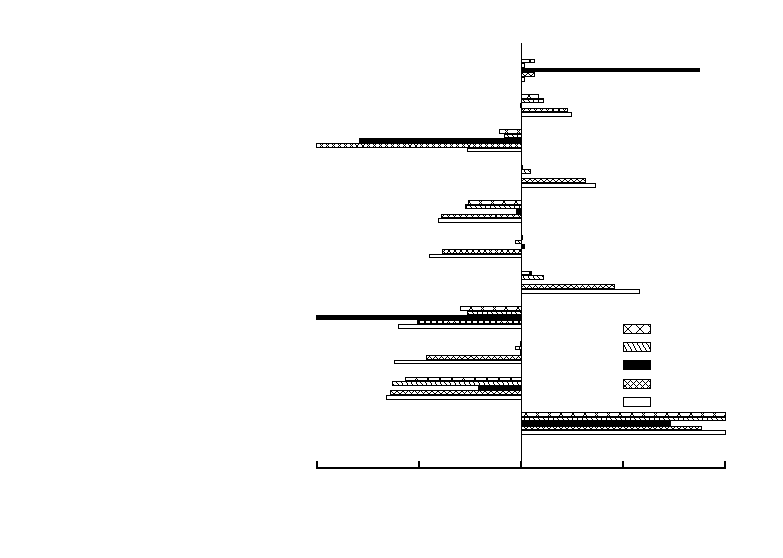
\includegraphics{CEMA_800}}%
    \gplfronttext
  \end{picture}%
\endgroup

  % GNUPLOT: LaTeX picture with Postscript
\begingroup
  \makeatletter
  \providecommand\color[2][]{%
    \GenericError{(gnuplot) \space\space\space\@spaces}{%
      Package color not loaded in conjunction with
      terminal option `colourtext'%
    }{See the gnuplot documentation for explanation.%
    }{Either use 'blacktext' in gnuplot or load the package
      color.sty in LaTeX.}%
    \renewcommand\color[2][]{}%
  }%
  \providecommand\includegraphics[2][]{%
    \GenericError{(gnuplot) \space\space\space\@spaces}{%
      Package graphicx or graphics not loaded%
    }{See the gnuplot documentation for explanation.%
    }{The gnuplot epslatex terminal needs graphicx.sty or graphics.sty.}%
    \renewcommand\includegraphics[2][]{}%
  }%
  \providecommand\rotatebox[2]{#2}%
  \@ifundefined{ifGPcolor}{%
    \newif\ifGPcolor
    \GPcolortrue
  }{}%
  \@ifundefined{ifGPblacktext}{%
    \newif\ifGPblacktext
    \GPblacktexttrue
  }{}%
  % define a \g@addto@macro without @ in the name:
  \let\gplgaddtomacro\g@addto@macro
  % define empty templates for all commands taking text:
  \gdef\gplbacktext{}%
  \gdef\gplfronttext{}%
  \makeatother
  \ifGPblacktext
    % no textcolor at all
    \def\colorrgb#1{}%
    \def\colorgray#1{}%
  \else
    % gray or color?
    \ifGPcolor
      \def\colorrgb#1{\color[rgb]{#1}}%
      \def\colorgray#1{\color[gray]{#1}}%
      \expandafter\def\csname LTw\endcsname{\color{white}}%
      \expandafter\def\csname LTb\endcsname{\color{black}}%
      \expandafter\def\csname LTa\endcsname{\color{black}}%
      \expandafter\def\csname LT0\endcsname{\color[rgb]{1,0,0}}%
      \expandafter\def\csname LT1\endcsname{\color[rgb]{0,1,0}}%
      \expandafter\def\csname LT2\endcsname{\color[rgb]{0,0,1}}%
      \expandafter\def\csname LT3\endcsname{\color[rgb]{1,0,1}}%
      \expandafter\def\csname LT4\endcsname{\color[rgb]{0,1,1}}%
      \expandafter\def\csname LT5\endcsname{\color[rgb]{1,1,0}}%
      \expandafter\def\csname LT6\endcsname{\color[rgb]{0,0,0}}%
      \expandafter\def\csname LT7\endcsname{\color[rgb]{1,0.3,0}}%
      \expandafter\def\csname LT8\endcsname{\color[rgb]{0.5,0.5,0.5}}%
    \else
      % gray
      \def\colorrgb#1{\color{black}}%
      \def\colorgray#1{\color[gray]{#1}}%
      \expandafter\def\csname LTw\endcsname{\color{white}}%
      \expandafter\def\csname LTb\endcsname{\color{black}}%
      \expandafter\def\csname LTa\endcsname{\color{black}}%
      \expandafter\def\csname LT0\endcsname{\color{black}}%
      \expandafter\def\csname LT1\endcsname{\color{black}}%
      \expandafter\def\csname LT2\endcsname{\color{black}}%
      \expandafter\def\csname LT3\endcsname{\color{black}}%
      \expandafter\def\csname LT4\endcsname{\color{black}}%
      \expandafter\def\csname LT5\endcsname{\color{black}}%
      \expandafter\def\csname LT6\endcsname{\color{black}}%
      \expandafter\def\csname LT7\endcsname{\color{black}}%
      \expandafter\def\csname LT8\endcsname{\color{black}}%
    \fi
  \fi
  \setlength{\unitlength}{0.0500bp}%
  \begin{picture}(7200.00,5040.00)%
    \gplgaddtomacro\gplbacktext{%
      \csname LTb\endcsname%
      \put(2748,1043){\makebox(0,0)[r]{\strut{}CH$_3$OCH$_2$=CH$_2$O+CH$_3$}}%
      \put(2748,1383){\makebox(0,0)[r]{\strut{}CH$_3$OCH$_2$O$_2$=CH$_2$OCH$_2$O$_2$H}}%
      \put(2748,1722){\makebox(0,0)[r]{\strut{}CH$_3$OCH$_3$+CH$_3$=CH$_3$OCH$_2$+CH$_4$}}%
      \put(2748,2061){\makebox(0,0)[r]{\strut{}CH$_3$OCH$_3$+HO$_2$=CH$_3$OCH$_2$+H$_2$O$_2$}}%
      \put(2748,2400){\makebox(0,0)[r]{\strut{}CH$_3$+CH$_3$+M=C$_2$H$_6$+M}}%
      \put(2748,2740){\makebox(0,0)[r]{\strut{}CH$_3$+HO$_2$=CH$_3$O+OH}}%
      \put(2748,3079){\makebox(0,0)[r]{\strut{}CH$_3$+HO$_2$=CH$_4$+O$_2$}}%
      \put(2748,3418){\makebox(0,0)[r]{\strut{}CH$_2$OCH$_2$O$_2$H=OH+CH$_2$O+CH$_2$O}}%
      \put(2748,3757){\makebox(0,0)[r]{\strut{}H$_2$O$_2$+M=OH+OH+M}}%
      \put(2748,4097){\makebox(0,0)[r]{\strut{}H+O$_2$+M=HO$_2$+M}}%
      \put(2748,4436){\makebox(0,0)[r]{\strut{}H+O$_2$=O+OH}}%
      \put(2880,484){\makebox(0,0){\strut{}-1}}%
      \put(3861,484){\makebox(0,0){\strut{}-0.5}}%
      \put(4842,484){\makebox(0,0){\strut{} 0}}%
      \put(5822,484){\makebox(0,0){\strut{} 0.5}}%
      \put(6803,484){\makebox(0,0){\strut{} 1}}%
      \csname LTb\endcsname%
      \put(4841,154){\makebox(0,0){\strut{}Normalized Participation Index}}%
      \put(3076,1349){\makebox(0,0)[l]{\strut{}Point A}}%
      \put(3076,1518){\makebox(0,0)[l]{\strut{}Point B}}%
      \put(3076,1688){\makebox(0,0)[l]{\strut{}Point C}}%
      \put(3076,1857){\makebox(0,0)[l]{\strut{}Point D}}%
      \put(3076,2027){\makebox(0,0)[l]{\strut{}Point E}}%
      \put(3076,2231){\makebox(0,0)[l]{\strut{}$1100$ K}}%
    }%
    \gplgaddtomacro\gplfronttext{%
      \csname LTb\endcsname%
      \put(3532,1337){\makebox(0,0)[r]{\strut{} }}%
      \csname LTb\endcsname%
      \put(3532,1513){\makebox(0,0)[r]{\strut{} }}%
      \csname LTb\endcsname%
      \put(3532,1689){\makebox(0,0)[r]{\strut{} }}%
      \csname LTb\endcsname%
      \put(3532,1865){\makebox(0,0)[r]{\strut{} }}%
      \csname LTb\endcsname%
      \put(3532,2041){\makebox(0,0)[r]{\strut{} }}%
    }%
    \gplbacktext
    \put(0,0){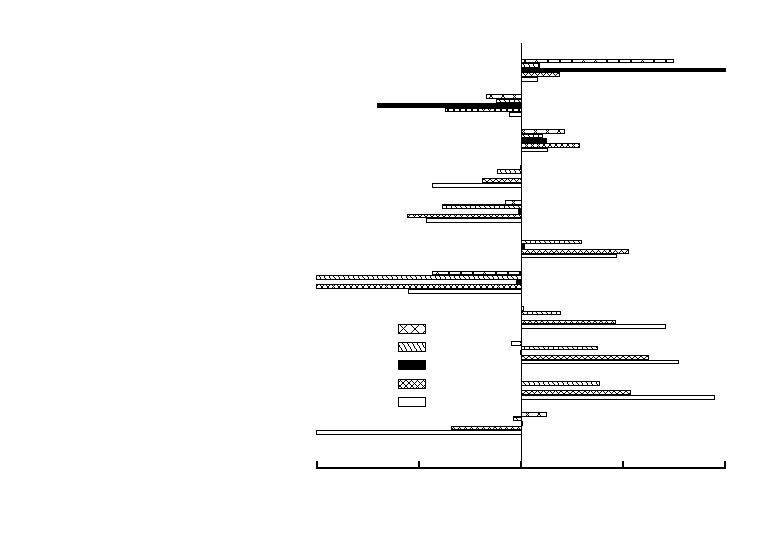
\includegraphics{CEMA_1100}}%
    \gplfronttext
  \end{picture}%
\endgroup

  \normalsize
  \caption{Normalized participation index at $800$ K and $1100$ K.  Sampled locations are marked in Fig.~\ref{fig:HRR}.  \textcolor{red}{Reaction arrow.}}
  \label{fig:CEMA}
\end{figure}



The above species profile analysis and CEMA results have demonstrated that autoignition chemistry is crucial to the complex flame structure in $700$ to $900$ K cases.  This is expected to some extent, as the mixture is autoignited.  However, the role that autoignition plays in the stabilization still needs further investigation.  For instance, as the mixture autoignites and propagates upstream, the relative contribution of the autoignition and flame propagation to the steady flame structure is still unclear.  Furthermore, it is intriguing that the $1100$ K case seems to have weaker autoignition chemistry in front of the flame compared to lower temperature cases.  To isolate the autoignition from flame propagation, Lagrangian Flamelet Modeling was performed.  The comparison between the one-dimensional flamelet solution and the two-dimensional CFD simulation would be able to demonstrate the dominating stabilization mechanism.  As if the thermal structure is stabilized by autoignition, following the mixture fraction iso-contour, the spatial information from the two-dimensional simulation could be interpreted as the time history of the corresponding mixture and predicted by the evolution of the flamelet.  Conversely, if flame propagation is the dominating stabilization mechanism, the flamelet solution would not agree well with the CFD simulation, since the transport processes along the mixture fraction iso-contour is not negligible compared to the gradient direction.

As mentioned in Sec.~\ref{sec:LFM}, the time history of the dissipation rate $\chi_{\rm st}$ was specified to FlameMaster according to the NGA simulation.  To avoid the ill-defined time in the recirculation zone, the time zero was defined at the location ten times of the fuel injector wall thickness downstream of the injector exit.  Accordingly, the species and temperature profiles along the transection at this location were specified as the initial conditions for the flamelet.  \textcolor{blue}{Furthermore, as the dissipation rate increases significantly across the flame, an extrapolation of $\chi_{\rm st}$ was made based on its time history profile prior to the flame to avoid the pollution from the NGA simulation.}  Based on these initial conditions and $\chi_{\rm st}$ time history profile, the unsteady flamelets were calculated and compared with the two-dimensional simulation results for $Z_{\rm st}$, $Z = 0.2$, and $Z = 0.3$.       
\begin{figure}
  \centering
  \scriptsize
  \input{LFM.tex}
%  % GNUPLOT: LaTeX picture with Postscript
\begingroup
  \makeatletter
  \providecommand\color[2][]{%
    \GenericError{(gnuplot) \space\space\space\@spaces}{%
      Package color not loaded in conjunction with
      terminal option `colourtext'%
    }{See the gnuplot documentation for explanation.%
    }{Either use 'blacktext' in gnuplot or load the package
      color.sty in LaTeX.}%
    \renewcommand\color[2][]{}%
  }%
  \providecommand\includegraphics[2][]{%
    \GenericError{(gnuplot) \space\space\space\@spaces}{%
      Package graphicx or graphics not loaded%
    }{See the gnuplot documentation for explanation.%
    }{The gnuplot epslatex terminal needs graphicx.sty or graphics.sty.}%
    \renewcommand\includegraphics[2][]{}%
  }%
  \providecommand\rotatebox[2]{#2}%
  \@ifundefined{ifGPcolor}{%
    \newif\ifGPcolor
    \GPcolortrue
  }{}%
  \@ifundefined{ifGPblacktext}{%
    \newif\ifGPblacktext
    \GPblacktexttrue
  }{}%
  % define a \g@addto@macro without @ in the name:
  \let\gplgaddtomacro\g@addto@macro
  % define empty templates for all commands taking text:
  \gdef\gplbacktext{}%
  \gdef\gplfronttext{}%
  \makeatother
  \ifGPblacktext
    % no textcolor at all
    \def\colorrgb#1{}%
    \def\colorgray#1{}%
  \else
    % gray or color?
    \ifGPcolor
      \def\colorrgb#1{\color[rgb]{#1}}%
      \def\colorgray#1{\color[gray]{#1}}%
      \expandafter\def\csname LTw\endcsname{\color{white}}%
      \expandafter\def\csname LTb\endcsname{\color{black}}%
      \expandafter\def\csname LTa\endcsname{\color{black}}%
      \expandafter\def\csname LT0\endcsname{\color[rgb]{1,0,0}}%
      \expandafter\def\csname LT1\endcsname{\color[rgb]{0,1,0}}%
      \expandafter\def\csname LT2\endcsname{\color[rgb]{0,0,1}}%
      \expandafter\def\csname LT3\endcsname{\color[rgb]{1,0,1}}%
      \expandafter\def\csname LT4\endcsname{\color[rgb]{0,1,1}}%
      \expandafter\def\csname LT5\endcsname{\color[rgb]{1,1,0}}%
      \expandafter\def\csname LT6\endcsname{\color[rgb]{0,0,0}}%
      \expandafter\def\csname LT7\endcsname{\color[rgb]{1,0.3,0}}%
      \expandafter\def\csname LT8\endcsname{\color[rgb]{0.5,0.5,0.5}}%
    \else
      % gray
      \def\colorrgb#1{\color{black}}%
      \def\colorgray#1{\color[gray]{#1}}%
      \expandafter\def\csname LTw\endcsname{\color{white}}%
      \expandafter\def\csname LTb\endcsname{\color{black}}%
      \expandafter\def\csname LTa\endcsname{\color{black}}%
      \expandafter\def\csname LT0\endcsname{\color{black}}%
      \expandafter\def\csname LT1\endcsname{\color{black}}%
      \expandafter\def\csname LT2\endcsname{\color{black}}%
      \expandafter\def\csname LT3\endcsname{\color{black}}%
      \expandafter\def\csname LT4\endcsname{\color{black}}%
      \expandafter\def\csname LT5\endcsname{\color{black}}%
      \expandafter\def\csname LT6\endcsname{\color{black}}%
      \expandafter\def\csname LT7\endcsname{\color{black}}%
      \expandafter\def\csname LT8\endcsname{\color{black}}%
    \fi
  \fi
  \setlength{\unitlength}{0.0500bp}%
  \begin{picture}(7200.00,5040.00)%
    \gplgaddtomacro\gplbacktext{%
      \csname LTb\endcsname%
      \put(2748,1043){\makebox(0,0)[r]{\strut{}CH$_3$OCH$_2$=CH$_2$O+CH$_3$}}%
      \put(2748,1383){\makebox(0,0)[r]{\strut{}CH$_3$OCH$_2$O$_2$=CH$_2$OCH$_2$O$_2$H}}%
      \put(2748,1722){\makebox(0,0)[r]{\strut{}CH$_3$OCH$_3$+CH$_3$=CH$_3$OCH$_2$+CH$_4$}}%
      \put(2748,2061){\makebox(0,0)[r]{\strut{}CH$_3$OCH$_3$+HO$_2$=CH$_3$OCH$_2$+H$_2$O$_2$}}%
      \put(2748,2400){\makebox(0,0)[r]{\strut{}CH$_3$+CH$_3$+M=C$_2$H$_6$+M}}%
      \put(2748,2740){\makebox(0,0)[r]{\strut{}CH$_3$+HO$_2$=CH$_3$O+OH}}%
      \put(2748,3079){\makebox(0,0)[r]{\strut{}CH$_3$+HO$_2$=CH$_4$+O$_2$}}%
      \put(2748,3418){\makebox(0,0)[r]{\strut{}CH$_2$OCH$_2$O$_2$H=OH+CH$_2$O+CH$_2$O}}%
      \put(2748,3757){\makebox(0,0)[r]{\strut{}H$_2$O$_2$+M=OH+OH+M}}%
      \put(2748,4097){\makebox(0,0)[r]{\strut{}H+O$_2$+M=HO$_2$+M}}%
      \put(2748,4436){\makebox(0,0)[r]{\strut{}H+O$_2$=O+OH}}%
      \put(2880,484){\makebox(0,0){\strut{}-1}}%
      \put(3861,484){\makebox(0,0){\strut{}-0.5}}%
      \put(4842,484){\makebox(0,0){\strut{} 0}}%
      \put(5822,484){\makebox(0,0){\strut{} 0.5}}%
      \put(6803,484){\makebox(0,0){\strut{} 1}}%
      \csname LTb\endcsname%
      \put(4841,154){\makebox(0,0){\strut{}Normalized Participation Index}}%
      \put(3076,1349){\makebox(0,0)[l]{\strut{}Point A}}%
      \put(3076,1518){\makebox(0,0)[l]{\strut{}Point B}}%
      \put(3076,1688){\makebox(0,0)[l]{\strut{}Point C}}%
      \put(3076,1857){\makebox(0,0)[l]{\strut{}Point D}}%
      \put(3076,2027){\makebox(0,0)[l]{\strut{}Point E}}%
      \put(3076,2231){\makebox(0,0)[l]{\strut{}$1100$ K}}%
    }%
    \gplgaddtomacro\gplfronttext{%
      \csname LTb\endcsname%
      \put(3532,1337){\makebox(0,0)[r]{\strut{} }}%
      \csname LTb\endcsname%
      \put(3532,1513){\makebox(0,0)[r]{\strut{} }}%
      \csname LTb\endcsname%
      \put(3532,1689){\makebox(0,0)[r]{\strut{} }}%
      \csname LTb\endcsname%
      \put(3532,1865){\makebox(0,0)[r]{\strut{} }}%
      \csname LTb\endcsname%
      \put(3532,2041){\makebox(0,0)[r]{\strut{} }}%
    }%
    \gplbacktext
    \put(0,0){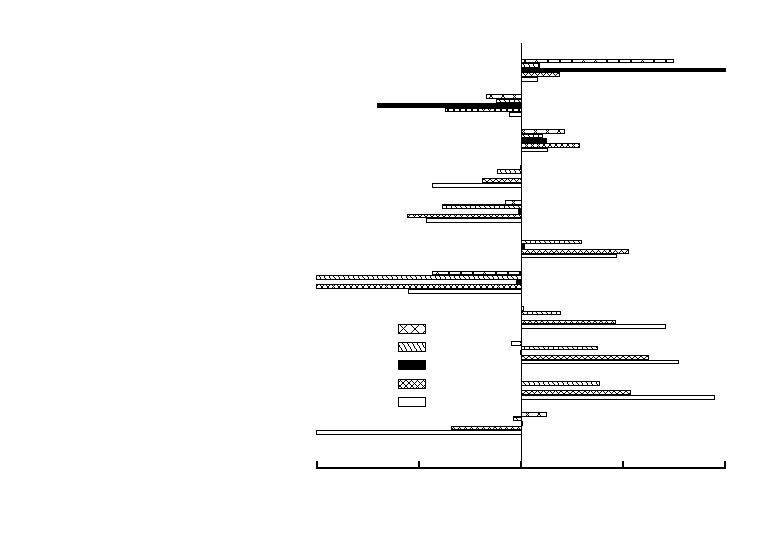
\includegraphics{CEMA_1100}}%
    \gplfronttext
  \end{picture}%
\endgroup

  \normalsize
  \vspace{0.2in}
  \caption{LFM \textcolor{red}{Set key}}
  \label{fig:LFM}
\end{figure}


As shown in Fig.~\ref{fig:LFM}, two ignition stages can be seen at $Z_{\rm st}$ and $Z = 0.2$ for the $700$ K case, while at $Z = 0.3$ only one ignition dominated by the low temperature chemistry is observed, due to the reduced initial temperature.   For the $800$ K case, both the flamelet and two-dimensional simulation experience almost identical time history, where two-stage ignition happens at all three mixture fractions.  As the initial temperatures further increase, corresponding to the increase in the boundary temperatures in the CFD simulation, the two-stage ignition phemonenon is less pronounced.  However, the $900$ K case still show good argeement between the flamelet autoignition profile with the time history of the two-dimensional simulation, similar to the above two cases.  

On the contrary, the ignition delay time computed with the one-dimensional flamelet assumption is significantly longer than the two-dimensional counterpart, indicating that autoignition is less important to the stabilization mechanism, and the transport processes along the mixture fraction iso-contours are important.  Although the dissipation rate other than $\chi_{\rm st}$ is computed through Eqn.~\ref{eqn:Zref}, and the time history profile is extrapolated, compared with the above three cases, the significant ignition delay suggests that flame propagation dominates the stabilization of the flame structure.       

With the above analysis based on species profiles, Chemical Explosive Mode Analysis, and Lagrangian Flamelet Model, the transition of the stabilization mechanism and the coupling between the autoignition chemistry and flame propagation can be clearly identified.  In the current study, two fundamental stabilization mechanisms are relevant: the \emph {kinetic} stabilization mechanism, due to the balance between the autoignition delay time and flow residence time, and the \emph {kinematic} stabilization mechanism, due to the balance between the premixed flame front propagation velocity and the local flow velocity.  On one hand, the stabilization mechanism depends on either balance achieved further upstream.  On the other hand, in this stratified composition and temperature field, autoignition and flame propagation processes are coupled through thermal and radical interactions, as the accumulation of the upstream radicals and heat release from autoignition accelerate the flame propagation velocity, and the flame transfers heat and radicals through back diffusion processes to the upstream, which could also facilitate autoignition.

\textcolor{blue}{The individual autoignition and flame propagation process reponds differently to the increasing boundary temperature.  The autoignition delay time behaves nonmonotonically, known as the NTC phenomenon, while the flame propagation velocity monotonically increases.  As a consequence, the flame structure is different from the classical triple flame, which is \emph{kinematically} stabilized, and the dominating stabilization mechanism alters.}   

For the current study, a purely \emph {kinetically} stabilized autoignition front was not observed, as all the stabilization points locate upstream of the ignition spot.  However, as demonstrated above, the \emph {kinetic} stabilization is the dominating mechanism for the $700$ to $900$ K cases.  Specifically, as seen from Fig.~\ref{fig:HRR}, the nonpremixed branch of the triple flame structure has quite low heat release rate for the $700$ K case, suggesting relatively weaker flame chemistry compared to autoignition.  As the boundary temperature increases to $800$ K, an autoignition front stabilizes the multibrachial structure at rich mixture fractions, due to shorter ignition delay time resulting from the NTC chemistry, and a modified triple flame structure anchors slightly downstream of this front at leaner mixture fractions.  Further increasing boundary temperature results in higher flame propagation velocity, therefore, the flame front at leaner mixture fraction depends less on the radicals accumulation ahead of the flame and propagates upstream, although the overall structure is still stabilized \emph {kinetically}.  The transition to a \emph {kinematically} stabilized flame structure is achieved as the $1100$ K case, where the flame propagation velocity balances the local incoming flow velocity, therefore, the flame structure stabilizes close to the injector exit and depends least on the radical accumulation from upstream.  

Based on the understanding obtained from the current study, further extension of the stabilization regime can be made, as shown in Fig.~\ref{fig:regime}.  As the inlet flow velocity is fixed, when the boundary temperature is sufficiently low, the mixture cannot be autoignited, and it is essentially the frozen flow.  Even external ignition source is applied, the flame cannot keep up with the excessive high flow velocity, such that the flame blows off.  When the boundary temperature is high enough to overcome the cold boundary difficulty, autoignition happens faraway downstream, and the flame propagation velocity still cannot keep up with the flow velocity.  As a consequence, a pure \emph {kinetically} stabilized autoignition front can be achieved.  Due to the computational cost to resolve such a large domain, the purely \emph {kinetically} stabilized case was not simulated.  Conversely, when the boundary temperature is sufficiently high, the autoignited flame propages fast upstream, where the flame chemistry is so strong that the upstream can be treated as frozen flow, which is similar to the $1100$ K case.  Therefore, a purely \emph {kinematically} stabilized classical triple flame structure is achieved.  Further increase in the boundary velocity results in an attached flame.  Although not included in the current paper, this attached flame was simulated at $1500$ K.  In between the purely \emph {kinetically} and \emph {kinematically} stabilized regime, there is a transitional regime governed by both mechanisms, which corresponds to the $700$ to $900$ K cases.  Due to the NTC behaviour of the autoignition chemistry, the stabilization point, in term of the mixture fraction space, varies, and the complex multibrachial flame structure appears.  

\begin{figure}[t]
  \centering
  \scriptsize
%  \vspace{-0.1in}
  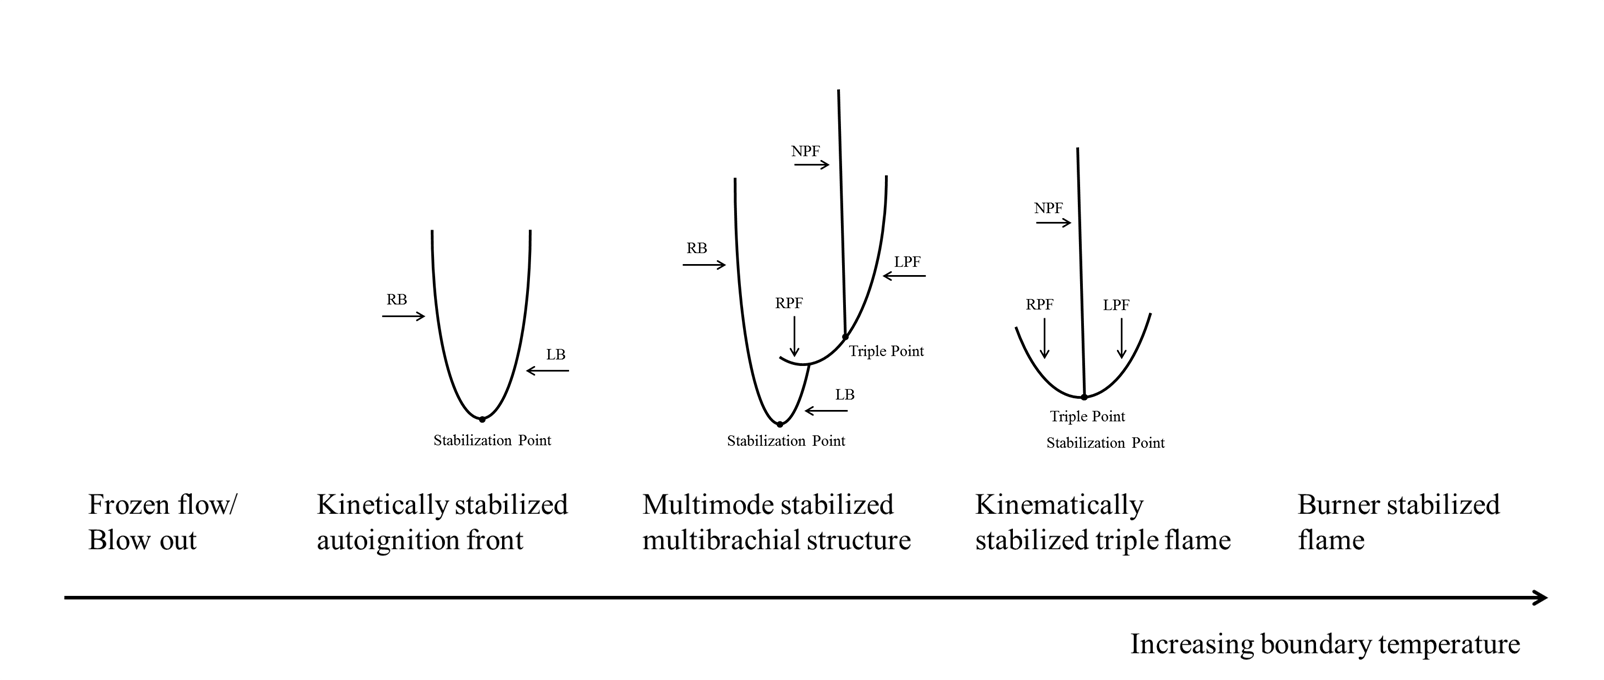
\includegraphics[width=1.0\textwidth]{regime.png}
  \normalsize
%  \vspace{-0.1in}
  \caption{Regime diagram of the stabilization mechanism as coflow boundary temperature increases.}
  \label{fig:regime}
\end{figure}

Further invesigations can be made to study parameters that modify the flame structure or autoignition front and the stabilization regime.  For example, boundary velocity can be varied to change the flow residence time, while dilution can be added to the fuel stream to change the chemical time scale.  Moreover, if autoignition is the dominating stabilization mechanism, and the dissipation rate is sufficiently low, the nonmonotonic lifted height variation can be observed as the boundary temperature changes, which is a plausible prediction based on the homogeneous autoignition and nonpremixed counterflow observation~\cite{deng14}.

\section{Conclusions}

In the present study, two-dimensional nonpremixed DME and heated air coflows were simulated using the NGA code.  The simulation was conducted under $30$ atmospheres to observe the influence of NTC chemistry on the stabilization mechanism.  DME was chosen as the fuel of interests, as it is practically an alternative biofuel for diesel engines, and well validated chemical models are available.  Uniform and fixed inlet boundary velocity was specified, and four coflow temperature ($700$, $800$, $900$, and $1100$ K) cases were studied.  The heat release rate profile, characteristic species profiles for low and high temperature chemistry, autoignition, and premixed flame propagation were examined.  Further investigation based on Chemical Explosive Mode Analysis and Lagrangian Flamelet Model enabled the determination of the stabilization mechanism.  

The $700$ to $900$ K cases were characterized as \emph {kinetically} stabilized, due to the dominating autoignition chemistry.  As the boundary temperature increases, the leading point of the heat release profile shifts to richer mixture fractions and then shifts back, due to the NTC effect in the autoignition process, and the coupling between the autoignition and premixed flame propagation chemistry.  

The $1100$ K case was characterized as \emph {kinematically} stabilized, as it preserves the classical triple flame structure, and the stabilization is achieved due to the balance between the premixed flame propagation velocity and the local incoming flow velocity.

Based on the current simulation results, extended stabilization regimes were identified.  For sufficiently high inlet velocity, as the boundary temperature increases from the cold case, frozen flow is firstly achieved, where the mixture cannot be autoignited, and even the flame generated by external ignition source will blow off.  When the mixture can be autoignited, the \emph {kinetically} stabilized autoignition front gradually transits to a \emph {kinematically} stabilized classical triple flame, where the premixed flame front propagation velocity balances the local incoming flow velocity.  The triple flame will eventually attach to the burner exit when the boundary temperature is sufficiently high.

Further study on the effects of fuel dilution and inlet velocity on the lifted height, stabilized flame structure, and stabilization mechanism, is suggested. 

\textcolor{red}{References.}

\end{document}

\section*{Acknowledgments}
This work was supported by the Combustion Energy Frontier Research Center, an Energy Frontier Research Center funded by the US Department of Energy, Office of Basic Energy Sciences under Award Number DE-SC0001198.

\section*{References}
\bibliographystyle{elsarticle-num-CNF}
\bibliography{DME_Jet}

\renewcommand{\thefigure}{\arabic{figure}}
\renewcommand{\thetable}{\arabic{table}}



  
